\chapter{同伦类型论 (Homotopy Type Theory)}
\label{cha:basics}

同伦类型论中的一个核心新观点是,可以将类型视为同伦理论中的空间或范畴论中的高维群胚(higher-dimensional groupoids)。

\index{classical!homotopy theory|(}
\index{higher category theory|(}
我们首先简要介绍同伦理论与高维范畴论之间的联系。
在经典同伦理论中,空间 $X$ 是一组带有拓扑结构的点集合,
\indexsee{space!topological}{topological space}
\index{topological!space}
而点 $x$ 和 $y$ 之间的路径通过一个连续映射 $p : [0,1] \to X$ 来表示,其中 $p(0) = x$ 和 $p(1) = y$。
\index{path!topological}
\index{topological!path}
这个函数可以被视为在每一个“时间点”提供 $X$ 中的一个点。对于许多目的而言,路径的严格相等(即逐点相等的函数)是一个过于精细的概念。例如,可以定义路径拼接操作(如果 $p$ 是从 $x$ 到 $y$ 的路径,$q$ 是从 $y$ 到 $z$ 的路径,那么拼接 $p \ct q$ 是从 $x$ 到 $z$ 的路径)和逆操作($\opp p$ 是从 $y$ 到 $x$ 的路径)。然而,这些操作之间存在自然的等式,但对于严格相等来说并不成立:例如,路径 $p \ct \opp p$(从 $x$ 走到 $y$,然后沿同一路径返回,时间从 $0$ 走到 $1$)并不严格等于恒等路径(在所有时间点都停留在 $x$ 处)。

解决方法是考虑一种称为\emph{同伦 (homotopy)}的路径相等的更粗略概念。
\index{homotopy!topological}
两个连续映射 $f : X_1 \to X_2$ 和 $g : X_1 \to X_2$ 之间的同伦是一个连续映射 $H : X_1 \times [0, 1] \to X_2$,满足 $H(x, 0) = f(x)$ 和 $H(x, 1) = g(x)$。在从 $x$ 到 $y$ 的路径 $p$ 和 $q$ 的特定情况下,同伦是一个连续映射 $H : [0,1] \times [0,1] \rightarrow X$,使得对所有 $s\in [0,1]$,$H(s,0) = p(s)$ 和 $H(s,1) = q(s)$。
在这种情况下,我们还要求对所有 $t\in [0,1]$,$H(0,t) = x$ 和 $H(1,t)=y$,以使得对每个 $t$,函数 $H(\blank,t)$ 再次是从 $x$ 到 $y$ 的路径;这种类型的同伦被称为\emph{端点保持 (endpoint-preserving)}或\emph{相对端点 (rel endpoints)}。
在简单的情况下,我们可以将 $H$ 的方形 $[0,1]\times [0,1]$ 的映像视为“填充”在 $p$ 和 $q$ 之间的空间,尽管对于一般的 $X$ 来说,这并不实际;更好的是将 $H$ 视为将 $p$ 连续变形为 $q$ 的过程,且不移动端点。
由于 $[0,1]\times [0,1]$ 是二维的,我们也可以称 $H$ 为路径之间的二维\emph{路径 (2-dimensional path)}。\index{path!2-}

例如,由于 $p \ct \opp p$ 沿同一路径来回走,你知道你可以将 $p \ct \opp p$ 连续缩小到恒等路径——例如,它不会被空间中的一个洞卡住。
同伦是一个等价关系,并且诸如拼接、逆操作等操作都尊重同伦。此外,在某个点 $x_0$ 处的闭环的同伦等价类(其中两个闭环 $p$ 和 $q$ 在它们之间存在\emph{基点保持 (based)}同伦时被等同,这是一种满足 $H(0,t) = H(1,t) = x_0$ 的同伦)形成一个称为\emph{基本群 (fundamental group)}的群。\index{fundamental!group}这个群是空间的一个\emph{代数不变量 (algebraic invariant)},可以用来调查两个空间是否\emph{同伦等价 (homotopy equivalent)}(存在来回连续映射且它们的复合是同伦于恒等映射的),因为等价空间具有同构的基本群。

由于同伦本身是一种二维路径,因此自然存在三维\emph{同伦之间的同伦 (homotopy between homotopies)}\index{path!3-},然后是\emph{同伦之间的同伦之间的同伦},依此类推。
这个由点、路径、同伦、同伦之间的同伦……所组成的无限塔,带有诸如基本群的代数操作,是一种称为\emph{(弱)$\infty$-群胚 (weak $\infty$-groupoid)}的代数结构。\index{.infinity-groupoid@$\infty$-groupoid} $\infty$-群胚\index{.infinity-groupoid@$\infty$-groupoid}包含一组对象,然后是对象之间的\emph{态射 (morphisms)}\indexdef{morphism!in an .infinity-groupoid@in an $\infty$-groupoid},然后是态射之间的\emph{态射},依此类推,并带有一些复杂的代数结构;在每一层级上的态射称为\define{$k$-态射 ($k$-morphism)}。\indexdef{k-morphism@$k$-morphism}每一层级的态射具有恒等、组合和逆操作,这些操作在某种意义上是弱的,即它们仅满足到下一层级的态射的群胚定律(组合的结合律、恒等是组合的单位元、逆元素消除),而这种弱性导致了进一步的结构。例如,由于组合的结合律 $p \ct (q \ct r) = (p \ct q) \ct r$ 本身是一种高维态射,因此需要额外的操作来关联各种结合律的证明:将 $p \ct (q \ct (r \ct s))$ 重新组合成 $((p \ct q) \ct r) \ct s$ 的各种方式产生了 Mac Lane 的五边形。\index{pentagon, Mac Lane}这种弱性还在各个层级之间产生了非平凡的相互作用。

每一个拓扑空间 $X$ 都具有一个\emph{基本$\infty$-群胚 (fundamental $\infty$-groupoid)},\index{.infinity-groupoid@$\infty$-groupoid!fundamental}\index{fundamental!.infinity-groupoid@$\infty$-groupoid}其 $k$-态射是 $X$ 中的 $k$维路径。$\infty$-群胚的弱性直接对应于路径仅同伦的事实,$(k+1)$-路径充当 $k$-路径之间的同伦。此外,将空间视为 $\infty$-群胚保持了足够的空间方面的特征以进行同伦理论:基本 $\infty$-群胚构造与 $\infty$-群胚作为空间的几何实现是伴随的,并且这种伴随保持了同伦理论(这被称为\emph{同伦假设/定理 (homotopy hypothesis/theorem)},\index{hypothesis!homotopy}\index{homotopy!hypothesis}因为它是一个假设还是定理取决于你如何定义 $\infty$-群胚)。例如,你可以很容易地定义一个 $\infty$-群胚的基本群,如果你计算一个空间的基本 $\infty$-群胚的基本群,它将与该空间的经典基本群的定义一致。由于这种对应关系,同伦理论与高维范畴论紧密相关。

\index{classical!homotopy theory|)}%
\index{higher category theory|)}%

\mentalpause

现在,在同伦类型论中,每一个类型都可以被视为具有 $\infty$-群胚的结构。回想一下,对于任何类型 $A$,以及任何 $x,y:A$,我们有一个等同性类型 $\id[A]{x}{y}$,也可以写作 $\idtype[A]{x}{y}$ 或简单地写作 $x=y$。从逻辑上讲,我们可以将 $\id[A]{x}{y}$ 的元素视为 $x$ 和 $y$ 相等的证据,或者是 $x$ 与 $y$ 的同一化(identification)。此外,类型论(不同于一阶逻辑)允许我们将 $\id[A]{x}{y}$ 的元素也视为可以成为进一步命题的对象的个体。因此,我们可以\emph{迭代}等同性类型:我们可以形成同一化 $p,q$ 之间的 $\id[{(\id[A]{x}{y})}]{p}{q}$ 类型,以及同一化 $r,s$ 之间的 $\id[{(\id[{(\id[A]{x}{y})}]{p}{q})}]{r}{s}$ 类型,依此类推。这种等同性类型的层级结构与空间中的连续路径及其之间的(更高阶)同伦,或一个 $\infty$-群胚的结构完全对应。\index{.infinity-groupoid@$\infty$-groupoid}

因此,我们经常将一个元素 $p : \id[A]{x}{y}$ 称为从 $x$ 到 $y$ 的\define{路径 (path)},\index{path}称 $x$ 为其\define{起点 (start point)},\indexdef{start point of a path}\indexdef{path!start point of}称 $y$ 为其\define{终点 (end point)}。\indexdef{end point of a path}\indexdef{path!end point of} 具有相同起点和终点的两条路径 $p,q : \id[A]{x}{y}$ 称为\define{平行 (parallel)},\indexdef{parallel paths}\indexdef{path!parallel}在这种情况下,元素 $r : \id[{(\id[A]{x}{y})}]{p}{q}$ 可以被视为同伦,或者是态射之间的态射;我们通常称它为\define{二维路径 (2-path)}\indexdef{path!2-}\indexsee{2-path}{path, 2-}或\define{二维路径 (2-dimensional path)}。\index{dimension!of paths}\indexsee{2-dimensional path}{path, 2-}\indexsee{path!2-dimensional}{path, 2-}类似地,$\id[{(\id[{(\id[A]{x}{y})}]{p}{q})}]{r}{s}$ 是\define{三维路径 (3-dimensional paths)}\indexdef{path!3-}\indexsee{3-path}{path, 3-}\indexsee{3-dimensional path}{path, 3-}\indexsee{path!3-dimensional}{path, 3-}的类型,用于两个平行二维路径之间的同一化。 如果类型 $A$ 是“类集(set-like)”的,如 \nat,这些迭代的等同性类型将变得无趣(参见 \cref{sec:basics-sets}),但在一般情况下,它们可以建模非平凡的同伦类型。

%% (显然,“$\id[A]{x}{y}$” 的符号在这里有其局限性。样式 $\idtype[A]{x}{y}$ 在迭代中只稍微好一些:$\idtype[{\idtype[{\idtype[A]{x}{y}}]{p}{q}}]{r}{s}$。)

同伦类型论与经典同伦理论之间的一个重要区别在于,同伦类型论提供了一种\emph{综合的 (synthetic)}描述空间的方式,\index{synthetic mathematics}\index{geometry, synthetic}\index{Euclid of Alexandria}如下所示。综合几何是欧几里得(Euclid)风格的几何学~\cite{Euclid}:从一些基本概念(点和线)、构造(连接任何两点的线)和公理(所有直角都相等)开始,逻辑地推导出结论。这与解析几何形成对比,\index{analytic mathematics}其中点和线等概念用 $\R^n$ 中的笛卡尔坐标具体表示——线是点集——并且基本的构造和公理源自这种表示。虽然经典同伦理论是解析性的(空间和路径是由点构成的),同伦类型论是综合性的:点、路径及路径之间的路径是基本的、不可分割的、原始的概念。

此外,同伦类型论的一个令人惊叹之处在于,所有基本的构造和公理——所有更高维的群胚结构——都自动从等同性类型的归纳原理中产生。
回想 \cref{sec:identity-types} 中的内容,该内容表明如果
\begin{itemize}
  \item 对于每个 $x,y:A$ 以及每个 $p:\id[A]xy$,我们有一个类型 $D(x,y,p)$,并且
  \item 对于每个 $a:A$,我们有一个元素 $d(a):D(a,a,\refl a)$,
\end{itemize}
那么
\begin{itemize}
  \item 对于\emph{每}个元素 $x,y:A$ 及 $p:\id[A]xy$,存在一个元素 $\indid{A}(D,d,x,y,p):D(x,y,p)$,使得 $\indid{A}(D,d,a,a,\refl a) \jdeq d(a)$。
\end{itemize}
换句话说,给定依赖函数
\begin{align*}
  D & :\prd{x,y:A} (\id{x}{y}) \to \type\\
  d & :\prd{a:A} D(a,a,\refl{a})
\end{align*}
存在一个依赖函数
\[\indid{A}(D,d):\prd{x,y:A}{p:\id{x}{y}} D(x,y,p)\]
使得
\begin{equation}\label{eq:Jconv}
\indid{A}(D,d,a,a,\refl{a})\jdeq d(a)
\end{equation}
对于每个 $a:A$。
通常,每当我们应用这个归纳规则时,我们要么不关心正在定义的特定函数,要么会立即给它一个不同的名称。

非正式地说,等同性类型的归纳原理表明,如果我们想要构造一个依赖于等同性类型的居住者 $p:\id[A]xy$ 的对象(或证明一个命题),那么仅在 $x$ 和 $y$ 是相同的(判断上的)且 $p$ 是反身元素 $\refl{x}:x=x$(判断上的)时进行构造(或证明)就足够了。
在非正式书写时,我们可能会用类似“通过归纳,可以假设……”的短语来表达这一点。
这种对“反身情况”的简化类似于在自然数上的归纳证明中的“基例”和“归纳步骤”的简化,也类似于在不交并或析取上的例证证明中的“左例证”和“右例证”的简化。\index{induction principle!for identity type}%

在自然数上的归纳证明的背景下,“转换规则”~\eqref{eq:Jconv} 并不常见,但在递归定义的相关概念中存在类似的概念。
如果一个序列 $(a_n)_{n\in \mathbb{N}}$ 是通过给定 $a_0$ 并根据 $a_n$ 指定 $a_{n+1}$ 来定义的,那么实际上生成序列的 $0^{\mathrm{th}}$ 项\emph{就是}给定的,并且给定的递推关系在生成的序列上成立。
(这似乎显而易见,不值得一提,但如果我们将递归定义视为计算序列值的算法\index{algorithm},那么这正是执行该算法的过程。)
规则~\eqref{eq:Jconv} 是类比的:它表明,如果我们通过指定当 $p$ 是 $\refl{x}:x=x$ 时的值来为所有 $p:x=y$ 定义一个对象 $f(p)$,那么我们指定的值实际上就是 $f(\refl{x})$ 的值。

这个归纳原理赋予每个类型 $\infty$-群胚\index{.infinity-groupoid@$\infty$-groupoid}的结构,并且每个类型之间的函数都具有 $\infty$-函子\index{.infinity-functor@$\infty$-functor}之间的函子的结构。这从数学的角度来看很有趣,因为它提供了一种处理 $\infty$-群胚的新方式。这从类型理论的角度来看也很有趣,因为它揭示了与每个类型和函数相关的新操作。在本章的其余部分,我们将开始探索这个结构。

\section{类型是高阶群体 (Types are higher groupoids)}
\label{sec:equality}

\index{类型!等同|(type!identity|(}%
\index{路径|(path|(}%
\index{.无穷群体@$\infty$-群体!类型的结构|(structure of a type|(}%
我们现在从归纳原理推导出高阶群体结构的开端。我们从等同的对称性开始,在拓扑语言中,这意味着“路径可以反向”。

\begin{lem}\label{lem:opp}
对于每一个类型 $A$ 和每一个 $x,y:A$,存在一个函数
\begin{equation*}
(x= y)\to(y= x)
\end{equation*}
记作 $p\mapsto \opp{p}$,使得对每一个 $x:A$,有 $\opp{\refl{x}}\jdeq\refl{x}$。我们称 $\opp{p}$ 为 $p$ 的 \define{逆元 (inverse)}。
\indexdef{路径!逆元 (path!inverse)}%
\indexdef{逆元!路径的 (inverse!of path)}%
\index{等同性!对称性 (equality!symmetry of)}%a
\index{对称性!等同性的 (symmetry!of equality)}%
\end{lem}

因为这是我们第一次声明某个东西为“引理”或“定理”,让我们停下来考虑一下这意味着什么。回想一下,命题(可以被证明的陈述)与类型等同,而引理和定理(已经被证明的陈述)与 \emph{居住的 (inhabited)} 类型等同。因此,引理或定理的陈述应被翻译成一个类型,如 \cref{sec:pat} 中那样,其证明被翻译成该类型的一个居住者。根据全称量词“对于每一个”的解释,\cref{lem:opp} 对应的类型是
\[ \prd{A:\UU}{x,y:A} (x= y)\to(y= x). \]
\cref{lem:opp} 的证明将包含构建该类型的一个元素,即推导出某个 $f:\prd{A:\UU}{x,y:A} (x= y)\to(y= x)$ 的判断。然后我们为这个元素 $f$ 引入符号 $\opp{(\blank)}$,其中 $A$、$x$ 和 $y$ 的参数被省略并从上下文推断。(如在 \cref{sec:types-vs-sets} 中所述,次要陈述“对于每一个 $x:A$,有 $\opp{\refl{x}}\jdeq\refl{x}$”应该被视为一个单独的判断。)

\begin{proof}[第一个证明 (First proof)]
  假设给定 $A:\UU$,
  令 $D:\prd{x,y:A}(x= y) \to \type$ 为由 $D(x,y,p)\defeq (y= x)$ 定义的类型族。换句话说,$D$ 是一个函数,将任意 $x,y:A$ 和 $p:x=y$ 分配给一个类型,即类型 $y=x$。然后我们有一个元素
  \begin{equation*}
    d\defeq \lam{x} \refl{x}:\prd{x:A} D(x,x,\refl{x}).
  \end{equation*}
  因此,身份类型的归纳原理给我们提供了一个元素
  \narrowequation{ \indid{A}(D,d,x,y,p): (y= x)}
  对于每个 $p:(x= y)$。我们现在可以定义所需的函数 $\opp{(\blank)}$ 为 $\lam{p} \indid{A}(D,d,x,y,p)$,即我们设 $\opp{p} \defeq \indid{A}(D,d,x,y,p)$。
  转换规则~\eqref{eq:Jconv} 给出 $\opp{\refl{x}}\jdeq \refl{x}$,如所需。
\end{proof}

我们以非常形式化的风格写出了这个证明,这在身份类型的归纳规则不熟悉时可能会有所帮助。为了更正式,我们可以说 \cref{lem:opp} 及其证明共同构成了以下判断
\begin{narrowmultline*}
  \lam{A}{x}{y}{p} \indid{A}((\lam{x}{y}{p} (y=x)), (\lam{x} \refl{x}), x, y, p)
  \narrowbreak : \prd{A:\UU}{x,y:A} (x= y)\to(y= x)
\end{narrowmultline*}
(以及额外的等同性判断)。然而,最终我们更喜欢使用更自然的语言,如以下等效的证明中那样。

\begin{proof}[第二个证明 (Second proof)]
  我们希望为每个 $x,y:A$ 和 $p:x=y$ 构造一个元素 $\opp{p}:y=x$。通过归纳,我们只需在 $y$ 为 $x$ 并且 $p$ 为 $\refl{x}$ 的情况下完成此操作。但在这种情况下,$p$ 的类型 $x=y$ 和我们试图构造 $\opp{p}$ 的类型 $y=x$ 都只是 $x=x$。因此,在“反射性情况”中,我们可以将 $\opp{\refl{x}}$ 简单地定义为 $\refl{x}$。然后通过归纳原理得出一般情况,并且转换规则 $\opp{\refl{x}}\jdeq\refl{x}$ 正是我们在反射性情况中给出的证明。
\end{proof}

我们将以这两种风格写出接下来的几个证明,以帮助读者熟悉后一种风格。接下来我们证明等同性的传递性,或等价地,我们“连接路径”。

\begin{lem}\label{lem:concat}
对于每一个类型 $A$ 和每一个 $x,y,z:A$,存在一个函数
\begin{equation*}
(x= y) \to   (y= z)\to (x=  z),
\end{equation*}
写作 $p \mapsto q \mapsto p\ct q$,使得对于任意 $x:A$,$\refl{x}\ct \refl{x}\jdeq \refl{x}$。
我们称 $p\ct q$ 为 $p$ 和 $q$ 的 \define{连接 (concatenation)} 或 \define{复合 (composite)}。
\indexdef{路径!连接 (path!concatenation)}%
\indexdef{路径!复合 (path!composite)}%
\indexdef{路径连接 (concatenation of paths)}%
\indexdef{路径的复合 (composition!of paths)}%
\index{等同性!传递性 (equality!transitivity of)}%
\index{传递性!等同性的 (transitivity!of equality)}%
\end{lem}

注意,我们选择以与函数复合相反的顺序来表示路径连接:从 $p:x=y$ 和 $q:y=z$ 我们得到 $p\ct q : x=z$,而从 $f:A\to B$ 和 $g:B\to C$ 我们得到 $g\circ f : A\to C$(见 \cref{ex:composition})。

\begin{proof}[第一个证明 (First proof)]
  所需的函数类型为 $\prd{x,y,z:A} (x= y) \to   (y= z)\to (x=  z)$。
  我们将定义一个具有等效类型的函数 $\prd{x,y:A} (x= y) \to \prd{z:A} (y= z)\to (x=  z)$,这允许我们进行两次路径归纳。令 $D:\prd{x,y:A} (x=y) \to \type$ 为类型族
  \begin{equation*}
    D(x,y,p)\defeq \prd{z:A}{q:y=z} (x=z)。
  \end{equation*}
  注意 $D(x,x,\refl x) \jdeq \prd{z:A}{q:x=z} (x=z)$。
  因此,为了将身份类型的归纳原理应用于此 $D$,我们需要一个类型为
  \begin{equation}\label{eq:concatD}
  \prd{x:A} D(x,x,\refl{x})
  \end{equation}
  的函数,即类型为
  \[ \prd{x,z:A}{q:x=z} (x=z)。\]
  现在令 $E:\prd{x,z:A}{q:x=z}\type$ 为类型族 $E(x,z,q)\defeq (x=z)$。
  注意 $E(x,x,\refl x) \jdeq (x=x)$。
  因此,我们有函数
  \begin{equation*}
    e(x) \defeq \refl{x} : E(x,x,\refl{x})。
  \end{equation*}
  通过身份类型的归纳原理应用于 $E$,我们得到一个函数
  \begin{equation*}
    d : \prd{x,z:A}{q:x=z} E(x,z,q)。
  \end{equation*}
  但是 $E(x,z,q)\jdeq (x=z)$,所以 $d$ 的类型是~\eqref{eq:concatD}。
  因此,我们可以使用此函数 $d$ 并将身份类型的归纳原理应用于 $D$,以获得我们所需的函数类型
  \begin{equation*}
    \prd{x,y:A} (x= y) \to \prd{z:A} (y= z)\to (x=  z)
  \end{equation*}
  因此 $\prd{x,y,z:A} (y=z) \to (x=y) \to (x=z)$。
  两个归纳原理的转换规则为任意 $x:A$ 给出了 $\refl{x}\ct \refl{x}\jdeq \refl{x}$。
\end{proof}

\begin{proof}[第二个证明 (Second proof)]
  我们希望为每个 $x,y,z:A$ 和每个 $p:x=y$ 和 $q:y=z$ 构造一个 $x=z$ 的元素。
  通过对 $p$ 进行归纳,我们只需假设 $y$ 是 $x$ 并且 $p$ 是 $\refl{x}$。
  在这种情况下,$q$ 的类型 $y=z$ 是 $x=z$。
  现在通过对 $q$ 进行归纳,我们只需再假设 $z$ 是 $x$ 并且 $q$ 是 $\refl{x}$。
  但在这种情况下,$x=z$ 是 $x=x$,我们有 $\refl{x}:(x=x)$。
\end{proof}

读者可能会觉得我们给出的这个引理证明过于复杂。实际上,我们可以在对 $p$ 进行归纳后停止,因为此时我们要生成的是一个等同 $x=z$,而我们已经有这样的等同,即 $q$。为什么我们还要继续对 $q$ 进行另一个归纳?

答案是,如介绍中所述,我们正在做的是 \emph{证明相关的 (proof-relevant)} 数学。
\index{数学!证明相关 (mathematics!proof-relevant)}%
当我们证明一个引理时,我们是在定义某个类型的一个居住者,并且在证明过程中定义的具体元素可能很重要,而不仅仅是该元素所居住的类型(即引理的 \emph{陈述})。\cref{lem:concat} 有三个显而易见的证明:我们可以对 $p$ 进行归纳,对 $q$ 进行归纳,或对它们进行双重归纳。如果我们用三种不同的方式证明它,我们将有三个相同类型的不同元素。不难证明这三个元素是相等的(见 \cref{ex:basics:concat}),但由于它们并非 \emph{定义上} 相等,因此可能仍有理由偏爱其中之一。

在 \cref{lem:concat} 的情况下,差异取决于计算规则。如果我们使用单一归纳对 $p$ 证明引理,那么我们将得到形式为 $\refl{y} \ct q \jdeq q$ 的计算规则。如果我们使用单一归纳对 $q$ 证明,那么我们将得到 $p\ct\refl{y}\jdeq p$,而我们用双重归纳(如我们所做的)证明则仅得到 $\refl{x}\ct\refl{x} \jdeq \refl{x}$。

\index{数学!形式化 (mathematics!formalized)}%
不对称的计算规则有时在做形式化数学时很方便,因为它们允许计算机自动简化更多内容。然而,在非正式数学中,甚至在形式化情况下,拥有一个表现不对称的连接操作并且必须记住哪个侧面是“特殊”的,可能会让人困惑。对两侧进行对称处理可以使证明更具稳健性;这就是为什么我们给出了我们所做的证明。(然而,这无疑是一个风格上的选择。)

下表总结了我们迄今为止所做的“等同性”、“同伦”和“高阶群体”的观点。
\begin{center}
  \medskip
  \begin{tabular}{ccc}
    \toprule
    等同性 (Equality) & 同伦 (Homotopy) & $\infty$-群体 ($\infty$-Groupoid)\\
    \midrule
    反射性\index{等同性!反射性 (equality!reflexivity of)} & 常量路径 & 恒等态射\\
    对称性\index{等同性!对称性 (equality!symmetry of)} & 路径反转 & 逆态射\\
    传递性\index{等同性!传递性 (equality!transitivity of)} & 路径连接 & 态射复合\\
    \bottomrule
  \end{tabular}
  \medskip
\end{center}

在实践中,传递性通常用于通过一系列中间步骤证明一个等同。我们将使用常见的符号表示,例如 $a=b=c=d$。如果中间表达式较长,或者我们想要指定每个等同的证据,我们可以写
\begin{align*}
  a &= b & \text{(由 $p$)}\\ &= c &\text{(由 $q$)} \\ &= d &\text{(由 $r$)}。
\end{align*}
在任何一种情况下,该符号表示构造元素 $(p\ct q)\ct r: (a=d)$。(为了具体化,我们选择左结合性,尽管考虑到 \cref{thm:omg}\ref{item:omg4},这几乎没有区别。)如果发生 $b$ 和 $c$ 是判断上相等的情况,那么我们可以写
\begin{align*}
  a &= b & \text{(由 $p$)}\\ &\jdeq c \\ &= d &\text{(由 $r$)}
\end{align*}
来表示构造 $p\ct r : (a=d)$。我们还遵循常见的数学实践,不要求该符号中的正当理由(“由 $p$”和“由 $r$”)提供所需的确切证据;相反,我们允许它们简单地提及构造该证据时最重要(或最不明显)的成分。例如,如果“引理 A”声明对于所有 $x$ 和 $y$ 我们有 $f(x)=g(y)$,那么我们可以写“由引理 A”作为步骤 $f(a) = g(b)$ 的正当理由,并相信读者能够推断出我们将引理 A 应用于 $x\defeq a$ 和 $y\defeq b$。如果我们相信读者能够猜出正当理由,我们也可以完全省略一个正当理由。

现在,由于证明相关性,我们不能在证明了等同性的“对称性”和“传递性”后停止:我们需要知道这些等同性操作是良好行为的。(这个问题在集合论中是看不见的,因为对称性和传递性只是等同性的 \emph{性质},而不是路径上的结构。)从同伦论的观点来看,连接和反转只是高阶群体结构的“第一级”——我们还需要这些操作的协调\index{协调 (coherence)}规律,以及更高维度的类似操作。例如,我们需要知道连接是 \emph{结合的 (associative)},并且反转提供了 \emph{连接的逆元 (inverses)}。

\begin{lem}\label{thm:omg}%[类型的 $\omega$-群体结构 (The $\omega$-groupoid structure of types)]
\index{路径连接的结合性 (associativity!of path concatenation)}%
\index{路径连接的单位律 (unit!law for path concatenation)}%
假设 $A:\type$,$x,y,z,w:A$ 并且 $p:x= y$,$q:y = z$ 和 $r:z=w$。
我们有以下内容:
\begin{enumerate}
  \item $p= p\ct \refl{y}$ 和 $p = \refl{x} \ct p$。\label{item:omg1}
  \item $\opp{p}\ct p=  \refl{y}$ 和 $p\ct \opp{p}= \refl{x}$。\label{item:omg2}
  \item $\opp{(\opp{p})}= p$。\label{item:omg3}
  \item $p\ct (q\ct r)=  (p\ct q)\ct r$。\label{item:omg4}
\end{enumerate}
\end{lem}

特别注意,\ref{item:omg1}--\ref{item:omg4} 本身是命题等同性,存在于身份类型 \emph{的} 身份类型中,例如 $p=_{x=y}q$ 对于 $p,q:x=y$。拓扑上,它们是 \emph{路径的路径 (paths of paths)},即同伦。在拓扑学中有一个熟悉的事实,当我们将路径 $p$ 与反转路径 $\opp p$ 连接时,我们不会字面上获得一个常量路径(对应于类型论中的等同性 $\refl{}$)——相反,我们有一个同伦或从 $p\ct\opp p$ 到常量路径的更高路径。

\begin{proof}[证明~\cref{thm:omg} (Proof of~\cref{thm:omg})]
  所有证明都使用身份等同的归纳原理。
  \begin{enumerate}
    \item \emph{第一个证明 (First proof):} 令 $D:\prd{x,y:A} (x=y) \to \type$ 为由
    \begin{equation*}
      D(x,y,p)\defeq (p= p\ct \refl{y})。
    \end{equation*}
    然后 $D(x,x,\refl{x})$ 是 $\refl{x}=\refl{x}\ct\refl{x}$。
    因为 $\refl{x}\ct\refl{x}\jdeq\refl{x}$,所以 $D(x,x,\refl{x})\jdeq (\refl{x}=\refl{x})$。
    因此,有一个函数
    \begin{equation*}
      d\defeq\lam{x} \refl{\refl{x}}:\prd{x:A} D(x,x,\refl{x})。
    \end{equation*}
    现在,身份类型的归纳原理为每个 $p:x= y$ 提供了一个元素 $\indid{A}(D,d,x,y,p):(p= p\ct\refl{y})$。
    另一个等同性的证明类似。

    \mentalpause

    \noindent
    \emph{第二个证明 (Second proof):} 通过对 $p$ 进行归纳,只需假设 $y$ 是 $x$ 并且 $p$ 是 $\refl x$。
    但在这种情况下,我们有 $\refl{x}\ct\refl{x}\jdeq\refl{x}$。
    \item \emph{第一个证明 (First proof):} 令 $D:\prd{x,y:A} (x=y) \to \type$ 为由
    \begin{equation*}
      D(x,y,p)\defeq (\opp{p}\ct p=  \refl{y})。
    \end{equation*}
    然后 $D(x,x,\refl{x})$ 是 $\opp{\refl{x}}\ct\refl{x}=\refl{x}$。
    因为 $\opp{\refl{x}}\jdeq\refl{x}$ 并且 $\refl{x}\ct\refl{x}\jdeq\refl{x}$,我们得到 $D(x,x,\refl{x})\jdeq (\refl{x}=\refl{x})$。
    因此,我们找到了函数
    \begin{equation*}
      d\defeq\lam{x} \refl{\refl{x}}:\prd{x:A} D(x,x,\refl{x})。
    \end{equation*}
    现在,路径归纳为每个 $p:x= y$ 提供了一个元素 $\indid{A}(D,d,x,y,p):\opp{p}\ct p=\refl{y}$。
    另一个等同性类似。

    \mentalpause

    \noindent \emph{第二个证明 (Second proof):} 通过归纳,只需假设 $p$ 是 $\refl x$。
    但在这种情况下,我们有 $\opp{p} \ct p \jdeq \opp{\refl x} \ct \refl x \jdeq \refl x$。

    \item \emph{第一个证明 (First proof):} 令 $D:\prd{x,y:A} (x=y) \to \type$ 为由
    \begin{equation*}
      D(x,y,p)\defeq (\opp{(\opp{p})}= p)。
    \end{equation*}
    然后 $D(x,x,\refl{x})$ 是类型 $(\opp{(\opp{\refl x})}=\refl{x})$。
    但因为 $\opp{\refl{x}}\jdeq \refl{x}$ 对于每个 $x:A$,我们有 $\opp{(\opp{\refl{x}})}\jdeq \opp{\refl{x}} \jdeq\refl{x}$,因此 $D(x,x,\refl{x})\jdeq(\refl{x}=\refl{x})$。
    因此,我们找到了函数
    \begin{equation*}
      d\defeq\lam{x} \refl{\refl{x}}:\prd{x:A} D(x,x,\refl{x})。
    \end{equation*}
    现在,路径归纳为每个 $p:x= y$ 提供了一个元素 $\indid{A}(D,d,x,y,p):\opp{(\opp{p})}= p$。

    \mentalpause

    \noindent \emph{第二个证明 (Second proof):} 通过归纳,只需假设 $p$ 是 $\refl x$。
    但在这种情况下,我们有 $\opp{(\opp{p})}\jdeq \opp{(\opp{\refl x})} \jdeq \refl x$。

    \item \emph{第一个证明 (First proof):} 令 $D_1:\prd{x,y:A} (x=y) \to \type$ 为由
    \begin{equation*}
      D_1(x,y,p)\defeq\prd{z,w:A}{q:y= z}{r:z= w} \big(p\ct (q\ct r)=  (p\ct q)\ct r\big)。
    \end{equation*}
    然后 $D_1(x,x,\refl{x})$ 是
    \begin{equation*}
      \prd{z,w:A}{q:x= z}{r:z= w} \big(\refl{x}\ct(q\ct r)= (\refl{x}\ct q)\ct r\big)。
    \end{equation*}
    要构造此类型的元素,令 $D_2:\prd{x,z:A} (x=z) \to \type$ 为类型族
    \begin{equation*}
      D_2 (x,z,q) \defeq \prd{w:A}{r:z=w} \big(\refl{x}\ct(q\ct r)= (\refl{x}\ct q)\ct r\big)。
    \end{equation*}
    然后 $D_2(x,x,\refl{x})$ 是
    \begin{equation*}
      \prd{w:A}{r:x=w} \big(\refl{x}\ct(\refl{x}\ct r)= (\refl{x}\ct \refl{x})\ct r\big)。
    \end{equation*}
    要构造 \emph{此} 类型的元素,令 $D_3:\prd{x,w:A} (x=w) \to \type$ 为类型族
    \begin{equation*}
      D_3(x,w,r) \defeq \big(\refl{x}\ct(\refl{x}\ct r)= (\refl{x}\ct \refl{x})\ct r\big)。
    \end{equation*}
    然后 $D_3(x,x,\refl{x})$ 是
    \begin{equation*}
      \big(\refl{x}\ct(\refl{x}\ct \refl{x})= (\refl{x}\ct \refl{x})\ct \refl{x}\big)
    \end{equation*}
    它在定义上等同于类型 $(\refl{x} = \refl{x})$,因此由 $\refl{\refl{x}}$ 居住。通过三次应用路径归纳规则,我们因此得到了整体所需类型的一个元素。

    \mentalpause

    \noindent \emph{第二个证明 (Second proof):} 通过归纳,只需假设 $p$、$q$ 和 $r$ 都是 $\refl x$。
    但在这种情况下,我们有
    \begin{align*}
      p\ct (q\ct r)
      &\jdeq \refl{x}\ct(\refl{x}\ct \refl{x})\\
      &\jdeq \refl{x}\\
      &\jdeq (\refl{x}\ct \refl x)\ct \refl x\\
      &\jdeq (p\ct q)\ct r。
    \end{align*}
    因此,我们有 $\refl{\refl{x}}$ 居住此类型。 \qedhere
  \end{enumerate}
\end{proof}

\begin{rmk}
  还有其他方式可以定义这些高阶路径。例如,在 \cref{thm:omg}\ref{item:omg4} 中,我们可能只对一条或两条路径进行归纳,而不是对所有三条路径进行归纳。每种可能性都会产生一个 \emph{定义上} 不同的证明,但它们都会相互等同。这种相互之间的等同性可以再次通过归纳证明,将所涉及的所有路径简化为反身性,然后观察到两个证明都简化为反身性。
\end{rmk}

根据 \cref{thm:omg}\ref{item:omg4},我们通常将 $p\ct q\ct r$ 写作 $(p\ct q)\ct r$,类似地,将 $p\ct q\ct r \ct s$ 写作 $((p\ct q)\ct r)\ct s$ 等。我们出于明确性的目的选择左结合性,但这并没有实际影响。我们通常相信读者能够根据需要插入 \cref{thm:omg}\ref{item:omg4} 的实例,以便重新关联此类表达式。

我们还没有真正完成高阶群体结构:路径~\ref{item:omg1}--\ref{item:omg4} 还必须满足它们自己的高阶协调\index{协调 (coherence)} 规律,这些规律本身是高阶路径,
\index{路径连接的结合性!协调性 (associativity!of path concatenation!coherence of)}%
\index{球形操作代数 (globular operad)}%
\index{操作代数 (operad)}%
\index{群体!高阶 (groupoid!higher)}%
依此类推,直到“无穷大”(这可以通过例如球形操作代数的概念来精确化)。然而,对于大多数目的来说,没有必要明确化整个无限维结构。同伦类型论的一个优点是,所有这些结构都可以从身份类型的归纳性质出发证明,因此我们可以根据需要显式化这些结构。

特别是,在本书中我们将不需要明确化所有高阶层次的复杂组合学。除了普通路径,我们将使用路径的路径(即类型 $p =_{x=_A y} q$ 的元素),如前面提到的,我们称之为 \emph{2-路径 (2-paths)} 或 \emph{2维路径 (2-dimensional paths)},也许偶尔使用路径的路径的路径(即类型 $r = _{p =_{x=_A y} q} s$ 的元素),我们称之为 \emph{3-路径 (3-paths)} 或 \emph{3维路径 (3-dimensional paths)}。定义一般的 \emph{$n$-维路径 ($n$-dimensional path)} 的概念是可能的
\indexdef{路径!n维@$n$- (path!n-@$n$-)}%
\indexsee{n-路径 (n-path@$n$-path)}{路径, $n$- (path, $n$-)}%
\indexsee{n维路径 (n-dimensional path@$n$-dimensional path)}{路径, $n$- (path, $n$-)}%
\indexsee{路径!n维@$n$-维}{路径, $n$- (path, $n$-)}%
(见 \cref{ex:npaths}),但我们将不需要它。

然而,我们将使用一种特别重要且简单的高阶路径情况,即起点和终点相同的情况。在集合论中,命题 $a=a$ 完全没有趣味,但在同伦论中,从一点到自身的路径称为 \emph{环路 (loops)} 并且包含了许多有趣的高阶结构。因此,给定一个具有点 $a:A$ 的类型 $A$,我们定义其 \define{环空间 (loop space)}
\index{环空间 (loop space)}%
$\Omega(A,a)$ 为类型 $\id[A]{a}{a}$。如果点 $a$ 从上下文中可以理解,我们有时可能会简单地写作 $\Omega A$。

由于 $\Omega A$ 的任意两个元素是具有相同起点和终点的路径,它们可以连接;
因此我们有一个操作 $\Omega A\times \Omega A\to \Omega A$。
更一般地,$A$ 的高阶群体结构赋予 $\Omega A$ 类似的“高阶群体”结构。

考虑 $A$ 的环空间的 \emph{环空间 (loop space)} 也很有用,这是在点 $a$ 上的单位环的 2维环空间。它写作 $\Omega^2(A,a)$,在类型论中表示为类型 $\id[({\id[A]{a}{a}})]{\refl{a}}{\refl{a}}$。
虽然 $\Omega^2(A,a)$ 作为一个环空间,再次是一个“高阶群体”,但由于其元素是 1维环上 2维环,这个环空间现在也有了一些附加结构。

\begin{thm}[埃克曼--希尔顿 (Eckmann--Hilton)]\label{thm:EckmannHilton}
第二环空间的组合操作
%
\begin{equation*}
  \Omega^2(A)\times \Omega^2(A)\to \Omega^2(A)
\end{equation*}
是可交换的:$\alpha\ct\beta = \beta\ct\alpha$,对于任意 $\alpha, \beta:\Omega^2(A)$。
\index{埃克曼--希尔顿论证 (Eckmann--Hilton argument)}%
\end{thm}

\begin{proof}
  首先,观察到 $1$-环的组合 $\Omega A\times \Omega A\to \Omega A$ 引入了一个操作
  \[
    \star : \Omega^2(A)\times \Omega^2(A)\to \Omega^2(A)
  \]
  如下:考虑元素 $a, b, c : A$ 和 1维及2维路径,
%
  \begin{align*}
    p &: a = b,       &       r &: b = c \\
    q &: a = b,       &       s &: b = c \\
    \alpha &: p = q,  &   \beta &: r = s
  \end{align*}
%
  如以下图所示(路径表示为箭头)。
% 为了具有统一的源代码,将此更改为 xymatrix,
% 也许原始使用的 xy 看起来更好(我认为它太大了)。
% 它在下面被注释掉,以防您想恢复它。
  \[
    \xymatrix@+5em{
        {a} \rtwocell<10>^p_q{\alpha}
      &
        {b} \rtwocell<10>^r_s{\beta}
      &
        {c}
    }
  \]
  分别连接上下的 1维路径,我们得到两个路径 $p\ct r,\ q\ct s : a = c$,然后在它们之间有一个“水平组合”
%
  \begin{equation*}
    \alpha\hct\beta : p\ct r = q\ct s
  \end{equation*}
%
  如下定义。
  首先,通过对 $r$ 进行路径归纳,我们定义 $\alpha \rightwhisker r : p\ct r = q\ct r$,使得
  \[ \alpha \rightwhisker \refl{b} \jdeq \opp{\mathsf{ru}_p} \ct \alpha \ct \mathsf{ru}_q \]
  其中 $\mathsf{ru}_p : p = p \ct \refl{b}$ 是来自 \cref{thm:omg}\ref{item:omg1} 的右单位律。
  我们可以类似地通过对 $\alpha$ 进行归纳,或者对视线中的所有路径进行归纳来定义 $\rightwhisker$,从而产生不同的判断等同,但对于当前目的,通过对 $r$ 进行归纳定义将使事情变得更简单。类似地,我们定义 $q\leftwhisker \beta : q\ct r = q\ct s$ 通过对 $q$ 进行归纳,使得
  \[ \refl{b} \leftwhisker \beta \jdeq \opp{\mathsf{lu}_r} \ct \beta \ct \mathsf{lu}_s \]
  其中 $\mathsf{lu}_r$ 表示左单位律。
  操作 $\leftwhisker$ 和 $\rightwhisker$ 被称为 \define{胡须 (whiskering)}\indexdef{胡须 (whiskering)}。
  接下来,由于 $\alpha \rightwhisker r$ 和 $q\leftwhisker \beta$ 是可组合的 2维路径,我们可以定义 \define{水平组合 (horizontal composition)}
  \indexdef{路径的水平组合 (horizontal composition!of paths)}%
  \indexdef{组合!路径的!水平 (composition!of paths!horizontal)}%
  为:
  \[
    \alpha\hct\beta\ \defeq\ (\alpha\rightwhisker r) \ct (q\leftwhisker \beta)。
  \]
  现在假设 $a \jdeq  b \jdeq  c$,因此所有 1维路径 $p$、$q$、$r$ 和 $s$ 都是 $\Omega(A,a)$ 的元素,并且进一步假设 $p\jdeq q \jdeq r \jdeq s\jdeq \refl{a}$,因此 $\alpha:\refl{a} = \refl{a}$ 和 $\beta:\refl{a} = \refl{a}$ 在两种顺序中都是可组合的。在这种情况下,我们有
  \begin{align*}
    \alpha\hct\beta
    &\jdeq (\alpha\rightwhisker\refl{a}) \ct (\refl{a}\leftwhisker \beta)\\
    &= \opp{\mathsf{ru}_{\refl{a}}} \ct \alpha \ct \mathsf{ru}_{\refl{a}} \ct \opp{\mathsf{lu}_{\refl a}} \ct \beta \ct \mathsf{lu}_{\refl{a}}\\
    &\jdeq \opp{\refl{\refl{a}}} \ct \alpha \ct \refl{\refl{a}} \ct \opp{\refl{\refl a}} \ct \beta \ct \refl{\refl{a}}\\
    &= \alpha \ct \beta。
  \end{align*}
  (回想一下,$\mathsf{ru}_{\refl{a}} \jdeq \mathsf{lu}_{\refl{a}} \jdeq \refl{\refl{a}}$,根据路径归纳的计算规则。)
  另一方面,我们可以通过类似方式定义另一个水平组合
  \[
    \alpha\hct'\beta\ \defeq\ (p\leftwhisker \beta)\ct (\alpha\rightwhisker s)
  \]
  并且我们类似地得出
  \[
    \alpha\hct'\beta = \beta\ct\alpha。
  \]
  \index{交换律 (interchange law)}%
  但是,通常情况下,定义水平组合的两种方式是相同的,$\alpha\hct\beta = \alpha\hct'\beta$,我们可以通过对 $\alpha$ 和 $\beta$ 进行归纳,然后对剩下的两条 1维路径进行归纳,将一切简化为反身性。
  因此我们有
  \[\alpha \ct \beta = \alpha\hct\beta = \alpha\hct'\beta = \beta\ct\alpha。
  \qedhere
  \]
\end{proof}

上述事实,被称为 \emph{埃克曼--希尔顿论证 (Eckmann--Hilton argument)},来自经典同伦论,实际上它在下面的 \cref{cha:homotopy} 中被用来证明类型的高阶同伦群总是阿贝尔\index{群!阿贝尔群 (group!abelian)}群。证明中定义的胡须和水平组合操作也是类型的 $\infty$-群体结构的一般部分。它们满足自己的规律(直到更高的同伦),例如
\[ \alpha \rightwhisker (p\ct q) = (\alpha \rightwhisker p) \rightwhisker q \]
等等。
从现在开始,我们相信读者在需要时应用路径归纳来定义此类进一步操作并验证其属性。

如本例所示,更高路径类型的代数比各个层次上的类似群体结构更为复杂;这些层次相互作用,产生许多进一步的操作和规律,如同伦论中迭代环空间的研究那样。事实上,如同经典同伦论,我们可以做出以下一般定义:

\begin{defn} \label{def:pointedtype}
一个 \define{带点类型 (pointed type)}
\indexsee{带点!类型 (pointed!type)}{类型, 带点 (type, pointed)}%
\indexdef{类型!带点 (type!pointed)}%
$(A,a)$ 是一个类型 $A:\type$,以及一个点 $a:A$,称为它的 \define{基点 (basepoint)}。
\indexdef{基点 (basepoint)}%
我们写作 $\pointed{\type} \defeq \sm{A:\type} A$ 来表示宇宙 $\type$ 中带点类型的类型。
\end{defn}

\begin{defn} \label{def:loopspace}
给定一个带点类型 $(A,a)$,我们定义其 \define{环空间 (loop space)}
\indexdef{环空间 (loop space)}%
为以下带点类型:
\[\Omega(A,a)\defeq ((\id[A]aa),\refl a)。\]
它的一个元素将被称为 $a$ 的 \define{环路 (loop)}。
对于 $n:\N$,$n$ 次迭代环空间的 \define{$n$-次迭代环空间 ($n$-fold iterated loop space)} $\Omega^{n}(A,a)$
\indexdef{环空间!迭代 (loop space!iterated)}%
\indexsee{环空间!n次迭代@$n$-次迭代 (loop space!n-fold@$n$-fold)}{环空间, 迭代 (loop space, iterated)}%
带点类型 $(A,a)$ 递归定义为:
\begin{align*}
  $\Omega^0(A,a)&\defeq(A,a)$\\
  $\Omega^{n+1}(A,a)&\defeq\Omega^n(\Omega(A,a))。
\end{align*}
它的一个元素将被称为 \define{$n$-环路 ($n$-loop)}
\indexdef{环路!n@$n$- (loop!n-@$n$-)}%
\indexsee{n环路 (n-loop@$n$-loop)}{环路, $n$- (loop, $n$-)}%
或 \define{$n$维环路 ($n$-dimensional loop)}
\indexsee{环路!n维@$n$维 (loop!n-dimensional@$n$-dimensional)}{环路, $n$- (loop, $n$-)}%
\indexsee{n维环路 (n-dimensional loop@$n$-dimensional loop)}{环路, $n$- (loop, $n$-)}%
在 $a$ 处。
\end{defn}

我们将在 \cref{cha:hlevels,cha:hits,cha:homotopy} 中回到迭代环空间。
\index{.无穷群体@$\infty$-群体!类型的结构|)}%
\index{类型!等同|)}%
\index{路径|)}%

\section{函数是函子 (Functions are functors)}
\label{sec:functors}

\index{函数 (function)|(}%
\index{类型论中函数的函子性@``类型论中函数的函子性'' (functoriality of functions in type theory)}%
我们现在希望证明函数 $f:A\to B$ 在路径上的行为是函子性的。在传统类型论中,这等价于函数尊重等同性的陈述。
\index{类型论中函数的连续性@``类型论中函数的连续性'' (continuity of functions in type theory)}%
从拓扑学的角度来看,这相当于说每个函数都是“连续的”,即保持路径的。

\begin{lem}\label{lem:map}
假设 $f:A\to B$ 是一个函数。
那么对于任意 $x,y:A$,存在一个操作
\begin{equation*}
\apfunc f : (\id[A] x y) \to (\id[B] {f(x)} {f(y)})。
\end{equation*}
此外,对于每个 $x:A$ 我们有 $\apfunc{f}(\refl{x})\jdeq \refl{f(x)}$。
\indexdef{函数应用于路径 (application!of function to a path)}%
\indexdef{路径!函数应用于路径 (path!application of a function to)}%
\indexdef{函数!应用于路径 (function!application to a path of)}%
\indexdef{函数在路径上的作用 (action!of a function on a path)}%
\end{lem}

符号 $\apfunc f$ 可以理解为 $f$ 对路径的 \underline{应用}(\underline{ap}plication),也可以理解为 $f$ 在路径上的 \underline{作用}(\underline{a}ction on \underline{p}aths)。

\begin{proof}[第一种证明 (First proof)]
令 $D:\prd{x,y:A} (x=y) \to \type$ 为定义为
\[D(x,y,p)\defeq (f(x)= f(y))。\]
的类型族。
然后我们有
\begin{equation*}
d\defeq\lam{x} \refl{f(x)}:\prd{x:A} D(x,x,\refl{x})。
\end{equation*}
通过路径归纳,我们得到 $\apfunc f : \prd{x,y:A} (x=y) \to (f(x)=f(y))$。
计算规则意味着对于每个 $x:A$,$\apfunc f({\refl{x}})\jdeq\refl{f(x)}$。
\end{proof}

\begin{proof}[第二种证明 (Second proof)]
要定义 $\apfunc{f}(p)$ 对于所有 $p:x=y$,通过归纳,假设
$p$ 是 $\refl{x}$ 就足够了。
在这种情况下,我们可以定义 $\apfunc f(p) \defeq \refl{f(x)}:f(x)= f(x)$。
\end{proof}

我们通常将 $\apfunc f (p)$ 简写为 $\ap f p$。
严格来说,这是模棱两可的,但通常不会引起混淆。
它符合范畴论中使用相同符号表示函子对对象和态射应用的常见约定。

我们注意到 $\apfunc{}$ 的行为是函子性的,以所有可能的方式体现了这一点。

\begin{lem}\label{lem:ap-functor}
对于函数 $f:A\to B$ 和 $g:B\to C$ 以及路径 $p:\id[A]xy$ 和 $q:\id[A]yz$,我们有:
\begin{enumerate}
\item $\apfunc f(p\ct q) = \apfunc f(p) \ct \apfunc f(q)$。\label{item:apfunctor-ct}
\item $\apfunc f(\opp p) = \opp{\apfunc f (p)}$。\label{item:apfunctor-opp}
\item $\apfunc g (\apfunc f(p)) = \apfunc{g\circ f} (p)$。\label{item:apfunctor-compose}
\item $\apfunc {\idfunc[A]} (p) = p$。
\end{enumerate}
\end{lem}
\begin{proof}
留给读者证明 (Left to the reader)。
\end{proof}
\index{函数 (function)|)}%

与 \cref{thm:omg} 中的等同性一样,\cref{lem:ap-functor} 中的等同性本身也是路径,这些路径满足它们自己的协调律(可以用同样的方法证明),依此类推。


\section{类型族是纤维化 (Type families are fibrations)}
\label{sec:fibrations}

\index{类型!族 (type!family of)|(}%
\index{传递 (transport)|(defstyle)}%
由于 \emph{依赖类型} 函数在类型论中是必不可少的,我们还需要 \cref{lem:map} 的一个版本。
然而,这并不容易表述,因为如果 $f:\prd{x:A} B(x)$ 且 $p:x=y$,那么 $f(x):B(x)$ 和 $f(y):B(y)$ 是属于不同类型的元素,因此 \emph{先验} 我们甚至不能询问它们是否相等。
缺少的成分是 $p$ 本身为我们提供了一种将类型 $B(x)$ 和 $B(y)$ 关联起来的方法。

我们已经在 \autoref{sec:identity-types} 中看到了这一点,我们称之为“相同者的不可分辨性 (indiscernibility of identicals)”。
\index{相同者的不可分辨性 (indiscernibility of identicals)}%
现在我们引入一个不同的名称和符号,之后我们将使用这个名称和符号。

\begin{lem}[传递 (Transport)]\label{lem:transport}
假设 $P$ 是一个在 $A$ 上的类型族,并且 $p:\id[A]xy$。
那么存在一个函数 $\transf{p}:P(x)\to P(y)$。
\end{lem}

\begin{proof}[第一种证明 (First proof)]
令 $D:\prd{x,y:A} (\id{x}{y}) \to \type$ 为定义为
\[D(x,y,p)\defeq P(x)\to P(y)。\]
的类型族。
然后我们有函数
\begin{equation*}
d\defeq\lam{x} \idfunc[P(x)] : \prd{x:A} D(x,x,\refl{x}),
\end{equation*}
因此归纳原理给我们 $p:x= y$ 时的 $\indid{A}(D,d,x,y,p):P(x)\to P(y)$,我们将其定义为 $\transf p$。
\end{proof}

\begin{proof}[第二种证明 (Second proof)]
通过归纳,假设 $p$ 是 $\refl x$ 就足够了。
但在这种情况下,我们可以将 $\transf{(\refl x)}:P(x)\to P(x)$ 视为恒等函数。
\end{proof}

有时,有必要标注传递操作发生的类型族 $P$。
在这种情况下,我们可以写作
\[\transfib P p \blank : P(x) \to P(y)。\]

回想一下,一个在类型 $A$ 上的类型族 $P$ 可以看作是 $A$ 的元素的一个性质,如果 $P(x)$ 是可居住的,则在 $A$ 中的 $x$ 处成立。
然后传递引理表明 $P$ 尊重等同性,在这种意义上,如果 $x$ 等于 $y$,那么 $P(x)$ 成立当且仅当 $P(y)$ 成立。
实际上,我们稍后将看到,如果 $x=y$,那么实际上 $P(x)$ 和 $P(y)$ 是 \emph{等价的}。

从拓扑学的角度来看,传递引理可以看作是纤维化中的“路径提升 (path lifting)”操作。
\index{纤维化 (fibration)}%
\indexdef{总空间 (total!space)}%
我们将类型族 $P:A\to \type$ 看作是一个基空间为 $A$ 的 \emph{纤维化},其中 $P(x)$ 是 $x$ 上的纤维,并且 $\sm{x:A}P(x)$ 是纤维化的 \define{总空间 (total space)},第一投影为 $\sm{x:A}(P(x))\to A$。
纤维化的定义属性是,在基空间 $A$ 中给定一条路径 $p:x=y$ 和纤维 $P(x)$ 上的一个点 $u$,我们可以将路径 $p$ 提升到总空间中以 $u$ 为起点的路径(并且这种提升可以连续地完成)。
可以认为点 $\trans p u$ 是这个提升路径的另一个端点。
我们也可以在类型论中定义路径本身:

\begin{lem}[路径提升属性 (Path lifting property)]\label{thm:path-lifting}
\indexdef{路径!提升 (path!lifting)}%
\indexdef{提升!路径 (lifting!path)}%
令 $P:A\to\type$ 为一个在 $A$ 上的类型族,并假设我们有 $u:P(x)$ 对于某个 $x:A$。
那么对于任意 $p:x=y$,我们有
\begin{equation*}
\mathsf{lift}(u,p):(x,u)=(y,\trans{p}{u})
\end{equation*}
在 $\sm{x:A}P(x)$ 中,使得 $\ap{\proj1}{\mathsf{lift}(u,p)} = p$。
\end{lem}
\begin{proof}
留给读者证明 (Left to the reader)。
我们将在 \cref{sec:compute-sigma} 中证明一个更一般的定理。
\end{proof}

在经典的同伦论中,纤维化被定义为一个映射,其中 \emph{存在} 路径的提升;而相对地,我们刚刚展示了在类型论中,每个类型族都带有一个 \emph{指定的} “路径提升函数”。
这符合构造性数学的哲学,根据该哲学,除非展示出它,否则我们不能表明某事存在。
\index{类型论中函数的连续性@``类型论中函数的连续性'' (continuity of functions in type theory)}%
它还自动确保路径提升是“连续地”选择的,因为正如我们所见,在类型论中所有函数都是“连续的”。

\begin{rmk}
尽管我们可能将类型族 $P:A\to \type$ 看作类似纤维化,但通常不建议说“纤维化 $P:A\to\type$”,因为这听起来像是在说基底是 $\type$ 而总空间是 $A$ 的纤维化。
再次强调,当一个类型族 $P:A\to \type$ 被看作纤维化时,基底是 $A$,而总空间是 $\sm{x:A} P(x)$。

我们也可能偶尔使用其他拓扑学术语来谈论类型族。
例如,我们可能将依赖函数 $f:\prd{x:A} P(x)$ 称为纤维化 $P$ 的 \define{截面 (section)}
\indexdef{类型族的截面 (section!of a type family)}%
,并且我们可能会说某事 \define{在纤维上 (fiberwise)} 发生
\indexdef{在纤维上 (fiberwise)}%
,如果它发生在每个 $P(x)$ 上。
例如,截面 $f:\prd{x:A} P(x)$ 表明 $P$ 是“在纤维上可居住的”。
\end{rmk}

\index{函数!依赖 (function!dependent)|(}
现在我们可以证明 \cref{lem:map} 的依赖版本。
拓扑学直觉是,假设 $f:\prd{x:A} P(x)$ 和路径 $p:\id[A]xy$,我们应该能够将 $f$ 应用于 $p$ 并在 $P$ 的总空间中获得一条“覆盖” $p$ 的路径,如下图所示。

\begin{center}
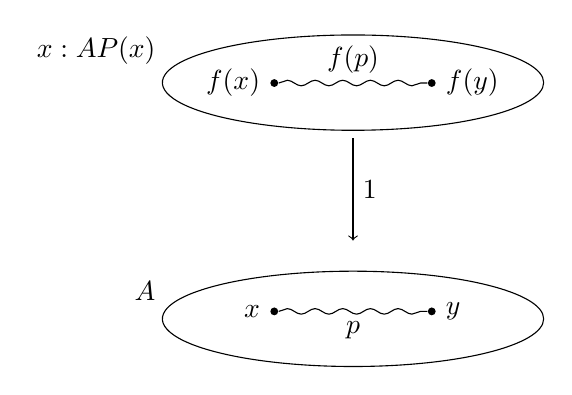
\begin{tikzpicture}[yscale=.5,xscale=2]
\draw (0,0) arc (-90:170:8ex) node[anchor=south east] {$A$} arc (170:270:8ex);
\draw (0,6) arc (-90:170:8ex) node[anchor=south east] {$\sm{x:A} P(x)$} arc (170:270:8ex);
\draw[->] (0,5.8) -- node[auto] {$\proj1$} (0,3.2);
\node[circle,fill,inner sep=1pt,label=left:{$x$}] (b1) at (-.5,1.4) {};
\node[circle,fill,inner sep=1pt,label=right:{$y$}] (b2) at (.5,1.4) {};
\draw[decorate,decoration={snake,amplitude=1}] (b1) -- node[auto,swap] {$p$} (b2);
\node[circle,fill,inner sep=1pt,label=left:{$f(x)$}] (b1) at (-.5,7.2) {};
\node[circle,fill,inner sep=1pt,label=right:{$f(y)$}] (b2) at (.5,7.2) {};
\draw[decorate,decoration={snake,amplitude=1}] (b1) -- node[auto] {$f(p)$} (b2);
\end{tikzpicture}
\end{center}

我们 \emph{可以} 从 \cref{lem:map} 中获得这样的结果。
给定 $f:\prd{x:A} P(x)$,我们可以通过设置 $f'(x)\defeq (x,f(x))$ 来定义一个非依赖函数 $f':A\to \sm{x:A} P(x)$,然后考虑 $\ap{f'}{p} : f'(x) = f'(y)$。
由于 $\proj1 \circ f' \jdeq \idfunc[A]$,通过 \cref{lem:ap-functor} 我们有 $\ap{\proj1}{\ap{f'}{p}} = p$;因此 $\ap{f'}{p}$ 确实在这个意义上“覆盖” $p$。
然而,从 \emph{类型} 的角度来看,$\ap{f'}{p}$ 并不明显覆盖 $A$ 中的任何特定路径(在本例中为 $p$),这在某些情况下可能很重要。

解决方案是使用传递引理。
根据 \cref{thm:path-lifting} 我们有一个从 $(x,u)$ 到 $(y,\trans p u)$ 的规范路径 $\mathsf{lift}(u,p)$,它覆盖 $p$。
因此,任何从 $u:P(x)$ 到 $v:P(y)$ 的路径覆盖 $p$ 应该通过 $\mathsf{lift}(u,p)$ 以基本唯一的方式在 $P(y)$ 的纤维中完全提升。
因此,直到等价性,定义“从 $u$ 到 $v$ 的路径覆盖 $p:x=y$”意义上意味着 $P(y)$ 中的路径 $\trans p u = v$ 是合理的。
而且,事实上,我们可以证明依赖函数会产生这样的路径。

\begin{lem}[依赖映射 (Dependent map)]\label{lem:mapdep}
\indexdef{依赖函数应用于路径 (application!of dependent function to a path)}%
\indexdef{路径!依赖函数应用于路径 (path!application of a dependent function to)}%
\indexdef{函数!依赖!应用于路径 (function!dependent!application to a path of)}%
\indexdef{依赖函数在路径上的作用 (action!of a dependent function on a path)}%
假设 $f:\prd{x: A} P(x)$;那么我们有一个映射
\[\apdfunc f : \prd{p:x=y}\big(\id[P(y)]{\trans p{f(x)}}{f(y)}\big)。\]
\end{lem}

\begin{proof}[第一种证明 (First proof)]
令 $D:\prd{x,y:A} (\id{x}{y}) \to \type$ 为定义为
\begin{equation*}
D(x,y,p)\defeq \trans p {f(x)}= f(y)。
\end{equation*}
的类型族。
然后 $D(x,x,\refl{x})$ 是 $\trans{(\refl{x})}{f(x)}= f(x)$。
但由于 $\trans{(\refl{x})}{f(x)}\jdeq f(x)$,我们得到 $D(x,x,\refl{x})\jdeq (f(x)= f(x))$。
因此,我们找到函数
\begin{equation*}
d\defeq\lam{x} \refl{f(x)}:\prd{x:A} D(x,x,\refl{x})
\end{equation*}
现在路径归纳为每个 $p:x= y$ 给我们 $\apdfunc f(p):\trans p{f(x)}= f(y)$。
\end{proof}

\begin{proof}[第二种证明 (Second proof)]
通过归纳,假设 $p$ 是 $\refl x$ 就足够了。
但在这种情况下,所需的等式是 $\trans{(\refl{x})}{f(x)}= f(x)$,这在判断上是成立的。
\end{proof}

我们通常将这种意义上“覆盖其他路径”的路径称为 \emph{依赖路径 (dependent paths)}。
\indexsee{依赖!路径 (dependent!path)}{路径, 依赖 (path, dependent)}%
\index{路径!依赖 (path!dependent)}%
它们将在 \cref{cha:hits} 中起到越来越重要的作用。
在 \cref{sec:computational} 中我们将看到,对于一些特定类型的类型族,有等价的方法来表示依赖路径的概念,这在某些情况下更为方便。

现在回想一下,在 \cref{sec:pi-types} 中,一个非依赖类型的函数 $f:A\to B$ 只是当 $P$ 是常量类型族 $P(x) \defeq B$ 时的依赖类型函数 $f:\prd{x:A} P(x)$ 的特例。
在这种情况下,$\apdfunc{f}$ 和 $\apfunc{f}$ 是密切相关的,因为有以下引理:

\begin{lem}\label{thm:trans-trivial}
如果 $P:A\to\type$ 定义为 $P(x) \defeq B$ 对于一个固定的 $B:\type$,那么对于任意 $x,y:A$ 和 $p:x=y$ 以及 $b:B$ 我们有路径
\[ \transconst Bpb : \transfib P p b = b。 \]
\end{lem}
\begin{proof}[第一种证明 (First proof)]
固定一个 $b:B$,令 $D:\prd{x,y:A} (\id{x}{y}) \to \type$ 为定义为
\[ D(x,y,p) \defeq (\transfib P p b = b)。\]
的类型族。
然后 $D(x,x,\refl x)$ 是 $(\transfib P{\refl{x}}{b} = b)$,根据传递的计算规则,这在判断上等于 $(b=b)$。
因此,我们有函数
\[ d \defeq \lam{x} \refl{b} : \prd{x:A} D(x,x,\refl x)。\]
现在路径归纳给我们一个
\narrowequation{
\prd{x,y:A}{p:x=y}(\transfib P p b = b),}
的元素,正如我们所希望的那样。
\end{proof}
\begin{proof}[第二种证明 (Second proof)]
通过归纳,假设 $y$ 是 $x$ 并且 $p$ 是 $\refl x$ 就足够了。
但是 $\transfib P {\refl x} b \jdeq b$,因此在这种情况下,我们要证明的是 $b=b$,并且我们有 $\refl{b}$ 可以证明。
\end{proof}

因此,对于任意 $x,y:A$ 和 $p:x=y$ 以及 $f:A\to B$,通过分别与 $\transconst Bp{f(x)}$ 及其逆连接,我们得到函数
\begin{align}
\big(f(x) = f(y)\big) &\to \big(\trans{p}{f(x)} = f(y)\big)\label{eq:ap-to-apd}
\qquad\text{和 (and)} \\
\big(\trans{p}{f(x)} = f(y)\big) &\to \big(f(x) = f(y)\big)。\label{eq:apd-to-ap}
\end{align}
实际上,这些函数是逆等价的(将在 \cref{sec:basics-equivalences} 中介绍),并且它们将 $\apfunc f (p)$ 与 $\apdfunc f (p)$ 关联起来。

\begin{lem}\label{thm:apd-const}
对于 $f:A\to B$ 和 $p:\id[A]xy$,我们有
\[ \apdfunc f(p) = \transconst B p{f(x)} \ct \apfunc f (p)。\]
\end{lem}
\begin{proof}[第一种证明 (First proof)]
令 $D:\prd{x,y:A} (\id xy) \to \type$ 为定义为
\[ D(x,y,p) \defeq \big(\apdfunc f (p) = \transconst Bp{f(x)} \ct \apfunc f (p)\big)。\]
的类型族。
因此,我们有
\[D(x,x,\refl x) \jdeq \big(\apdfunc f (\refl x) = \transconst B{\refl x}{f(x)} \ct \apfunc f ({\refl x})\big)。\]
但根据定义,这三个路径都是 $\refl{f(x)}$,所以我们有
\[ \refl{\refl{f(x)}} : D(x,x,\refl x)。\]
因此,路径归纳为我们提供了 $\prd{x,y:A}{p:x=y} D(x,y,p)$ 的元素,这正是我们想要的。
\end{proof}
\begin{proof}[第二种证明 (Second proof)]
通过归纳,假设 $y$ 是 $x$ 并且 $p$ 是 $\refl x$ 就足够了。
在这种情况下,我们要证明的是 $\refl{f(x)} = \refl{f(x)} \ct \refl{f(x)}$,这是在判断上成立的。
\end{proof}

由于 $\apdfunc{f}$ 和 $\apfunc{f}$ 的类型不同,通常使用不同的符号来表示它们会更清晰。
% 我们有时可能会使用符号 $\apd f p$ 表示 $\apdfunc{f}(p)$,类似于使用符号 $\ap f p$ 表示 $\apfunc{f}(p)$。

\index{函数!依赖 (function!dependent)|)}%

此时,我们希望读者开始熟悉身份类型的归纳证明。
从现在起,我们不再给出两种证明风格,而是允许我们使用最清晰和方便的证明(通常是第二种,更简洁的证明)。
以下是一些关于传递的有用引理;我们将其证明(采用任一风格)留给读者。

\begin{lem}\label{thm:transport-concat}
给定 $P:A\to\type$,其中 $p:\id[A]xy$ 和 $q:\id[A]yz$ 以及 $u:P(x)$,我们有
\[ \trans{q}{\trans{p}{u}} = \trans{(p\ct q)}{u}。 \]
\end{lem}

\begin{lem}\label{thm:transport-compose}
对于函数 $f:A\to B$ 和一个类型族 $P:B\to\type$,以及任意 $p:\id[A]xy$ 和 $u:P(f(x))$,我们有
\[ \transfib{P\circ f}{p}{u} = \transfib{P}{\apfunc f(p)}{u}。 \]
\end{lem}

\begin{lem}\label{thm:ap-transport}
对于 $P,Q:A\to \type$ 和一族函数 $f:\prd{x:A} P(x)\to Q(x)$,以及任意 $p:\id[A]xy$ 和 $u:P(x)$,我们有
\[ \transfib{Q}{p}{f_x(u)} = f_y(\transfib{P}{p}{u})。 \]
\end{lem}

\index{类型!族 (type!family of)|)}%
\index{传递 (transport)|)}

\section{同伦与等价 (Homotopies and equivalences)}
\label{sec:basics-equivalences}

\index{同伦 (homotopy)|(defstyle}%

到目前为止,我们已经看到,恒等类型 $\id[A]{x}{y}$ 可以被视为类型 $A$ 的两个元素 $x$ 和 $y$ 之间的 \emph{同一性 (identifications)}、\emph{路径 (paths)} 或 \emph{等价 (equivalences)} 的一种类型。
现在,我们探讨在 \emph{函数 (functions)} 和 \emph{类型 (types)} 之间``同一性''或``相同性''的适当概念。
在 \cref{sec:compute-pi,sec:compute-universe} 中,我们将看到,同伦类型论 (Homotopy Type Theory) 允许我们将这些与恒等类型的实例联系起来,但在此之前,我们需要独立理解它们。

传统上,如果两个函数在所有输入上都取相同的值,我们就认为它们是相同的。
根据命题即类型 (propositions-as-types) 的解释,这表明两个函数 $f$ 和 $g$(可能是依赖类型 (dependently typed) 的函数)是相同的,如果类型 $\prd{x:A} (f(x)=g(x))$ 是可居住的 (inhabited)。
根据同伦的解释,这种依赖函数类型由 \emph{连续 (continuous)} 路径或 \emph{函子等价 (functorial equivalences)} 组成,因此可以被视为 \emph{同伦 (homotopies)} 或 \emph{自然同构 (natural isomorphisms)} 的类型。\index{同构!自然 (isomorphism!natural)} 我们将采用拓扑学术语来表示这一点。

\begin{defn} \label{defn:homotopy}
设 $f,g:\prd{x:A} P(x)$ 是类型族 $P:A\to\type$ 的两个截面 (sections)。
从 $f$ 到 $g$ 的 \define{同伦 (homotopy)} 是一个依赖函数,类型为
\begin{equation*}
(f\htpy g) \defeq \prd{x:A} (f(x)=g(x)).
\end{equation*}
\end{defn}

请注意,同伦 (homotopy) 不等同于恒等 $(f=g)$。
然而,在 \cref{sec:compute-pi} 中,我们将引入一个公理,使得同伦和恒等``等价''。

以下证明留给读者。

\begin{lem}\label{lem:homotopy-props}
对于每个依赖函数类型 $\prd{x:A} P(x)$,同伦 (homotopy) 是一个等价关系 (equivalence relation)。
也就是说,我们有以下类型的元素:
\begin{gather*}
\prd{f:\prd{x:A} P(x)} (f\htpy f)\\
\prd{f,g:\prd{x:A} P(x)} (f\htpy g) \to (g\htpy f)\\
\prd{f,g,h:\prd{x:A} P(x)} (f\htpy g) \to (g\htpy h) \to (f\htpy h).
\end{gather*}
\end{lem}

% This is judgmental and is \cref{ex:composition}.
% \begin{lem}
%   Composition is associative and unital up to homotopy.
%   That is:
%   \begin{enumerate}
%   \item If $f:A\to B$ then $f\circ \idfunc[A]\htpy f\htpy \idfunc[B]\circ f$.
%   \item If $f:A\to B, g:B\to C$ and $h:C\to D$ then $h\circ (g\circ f) \htpy (h\circ g)\circ f$.
%   \end{enumerate}
% \end{lem}

\index{类型论中函数的函子性@``functoriality'' of functions in type theory}%
\index{类型论中函数的连续性@``continuity'' of functions in type theory}%
正如类型论 (type theory) 中的函数自动是``函子 (functors)''一样,同伦 (homotopies) 也自动是 \index{同伦的自然性@``naturality'' of homotopies} ``自然变换 (natural transformations)''。
我们将在此只对非依赖函数 $f,g:A\to B$ 进行说明和证明;在 \cref{ex:dep-htpy-natural} 中,我们要求读者将其推广到依赖函数。

回顾一下,对于 $f:A\to B$ 和 $p:\id[A]{x}{y}$,我们可以写 $\ap f p$ 表示 $\apfunc{f} (p)$。

\begin{lem}\label{lem:htpy-natural}
假设 $H:f\htpy g$ 是函数 $f,g:A\to B$ 之间的同伦,并且 $p:\id[A]{x}{y}$。那么我们有
\begin{equation*}
H(x)\ct\ap{g}{p}=\ap{f}{p}\ct H(y)。
\end{equation*}
我们也可以将其绘制为一个交换图 (commutative diagram):\index{图表 (diagram)}
\begin{align*}
\xymatrix{
f(x) \ar@{=}[r]^{\ap fp} \ar@{=}[d]_{H(x)} & f(y) \ar@{=}[d]^{H(y)} \\
g(x) \ar@{=}[r]_{\ap gp} & g(y)
}
\end{align*}
\end{lem}
\begin{proof}
通过归纳,我们可以假设 $p$ 是 $\refl{x}$。
由于 $\apfunc{f}$ 和 $\apfunc{g}$ 在反射性上计算,因此在这种情况下我们必须证明
\[ H(x) \ct \refl{g(x)} = \refl{f(x)} \ct H(x)。 \]
但这可以通过两边都等于 $H(x)$ 来证明。
\end{proof}

\begin{cor}\label{cor:hom-fg}
设 $H : f \htpy \idfunc[A]$ 是一个同伦,且 $f : A \to A$。那么对于任意 $x : A$,我们有 \[ H(f(x)) = \ap f{H(x)}。 \]
% The above path will be denoted by $\com{H}{f}{x}$.
\end{cor}
\noindent
这里 $f(x)$ 表示 $f$ 对 $x$ 的普通应用,而 $\ap f{H(x)}$ 表示 $\apfunc{f}(H(x))$。
\begin{proof}
根据 $H$ 的自然性,以下路径的图表是交换的:
\begin{align*}
\xymatrix@C=3pc{
ffx \ar@{=}[r]^-{\ap f{Hx}} \ar@{=}[d]_{H(fx)} & fx \ar@{=}[d]^{Hx} \\
fx \ar@{=}[r]_-{Hx} & x
}
\end{align*}
即 $\ap f{H x} \ct H x = H(f x) \ct H x$。
我们现在可以通过 $\opp{(H x)}$ 来操作以消去 $H x$,得到
\[ \ap f{H x}
= \ap f{H x} \ct H x \ct \opp{(H x)}
= H(f x) \ct H x \ct \opp{(H x)}
= H(f x)
\]
如所需 (其中一些结合性路径被忽略)。
\end{proof}

当然,像函数的函子性 (\cref{lem:ap-functor}) 一样,\cref{lem:htpy-natural} 中的等式是一个路径,它满足自己的相干性定律 (coherence laws) 等等。

\index{同伦 (homotopy)|)}%

\index{等价 (equivalence)|(}%
接下来是类型,从传统的角度来看,可以说一个函数 $f:A\to B$ 是一个 \emph{同构 (isomorphism)},如果存在一个函数 $g:B\to A$,使得两个复合 $f\circ g$ 和 $g\circ f$ 在点上等同于恒等函数 (identity function),即使得 $f \circ g \htpy \idfunc[B]$ 并且 $g\circ f \htpy \idfunc[A]$。
\indexsee{同伦!等价}{equivalence}%
从同伦的角度来看,这应该被称为 \emph{同伦等价 (homotopy equivalence)},而从范畴论 (categorical) 的角度来看,这应该被称为 \emph{高阶群 (higher groupoids) 的等价 (equivalence)}。
然而,在进行相关证明数学 (proof-relevant mathematics) 时,
\index{数学!相关证明 (mathematics!proof-relevant)}%
对应的类型
\begin{equation}
\sm{g:B\to A} \big((f \circ g \htpy \idfunc[B]) \times (g\circ f \htpy \idfunc[A])\big)\label{eq:qinvtype}
\end{equation}
表现不佳。
例如,对于单个函数 $f:A\to B$,可能存在多个不同的 \eqref{eq:qinvtype} 的不等价成员。
(这与高阶范畴理论 (higher category theory) 中的观察密切相关,即通常需要考虑 \emph{伴随等价 (adjoint equivalences)} \index{伴随!等价 (adjoint!equivalence)} 而不是普通的等价性)。
因此,我们给 \eqref{eq:qinvtype} 一个历史上准确的,但稍微贬义的名称。

\begin{defn}\label{defn:quasi-inverse}
对于一个函数 $f:A\to B$,$f$ 的 \define{拟逆 (quasi-inverse)} 是一个三元组 $(g,\alpha,\beta)$,由一个函数 $g:B\to A$ 和同伦 $\alpha:f\circ g\htpy \idfunc[B]$ 以及 $\beta:g\circ f\htpy \idfunc[A]$ 组成。
\end{defn}

\symlabel{qinv}
因此,\eqref{eq:qinvtype} 是 \emph{拟逆 (quasi-inverses) $f$ 的类型};我们可以用 $\qinv(f)$ 来表示它。

\begin{eg}\label{eg:idequiv}
\index{恒等!函数 (identity!function)}%
\index{函数!恒等 (function!identity)}%
恒等函数 $\idfunc[A]:A\to A$ 有一个拟逆,由 $\idfunc[A]$ 本身给出,以及同伦 $\alpha(y) \defeq \refl{y}$ 和 $\beta(x) \defeq \refl{x}$。
\end{eg}

\begin{eg}\label{eg:concatequiv}
对于任意 $p:\id[A]{x}{y}$ 和 $z:A$,函数
\begin{align*}
(p\ct \blank)&:(\id[A]{y}{z}) \to (\id[A]{x}{z}) \qquad\text{和}\\
(\blank \ct p)&:(\id[A]{z}{x}) \to (\id[A]{z}{y})
\end{align*}
具有拟逆 $(\opp p \ct \blank)$ 和 $(\blank \ct \opp p)$;见 \cref{ex:equiv-concat}。
\end{eg}

\begin{eg}\label{thm:transportequiv}
对于任意 $p:\id[A]{x}{y}$ 和 $P:A\to\type$,函数
\[\transfib{P}{p}{\blank}:P(x) \to P(y)\]
具有由 $\transfib{P}{\opp p}{\blank}$ 给出的拟逆;这可以从 \cref{thm:transport-concat} 中得到。
\end{eg}

\symlabel{basics-isequiv}\symlabel{basics:iso}
一般来说,我们只会在 $A$ 和 $B$ ``表现得像集合''的特殊情况下使用 \emph{同构 (isomorphism)}\index{同构!集合的 (isomorphism!of sets)}(以及类似的词汇如 \emph{双射 (bijection)},以及关联的符号 $A\cong B$)\index{双射 (bijection)}。
在这种情况下,类型 \eqref{eq:qinvtype} 是没有问题的。
我们将保留 \emph{等价 (equivalence)} 一词用于改进的概念 $\isequiv (f)$,具有以下性质:%
\begin{enumerate}
\item 对于每个 $f:A\to B$,存在一个函数 $\qinv(f) \to \isequiv (f)$。\label{item:be1}
\item 同样地,对于每个 $f$ 我们有 $\isequiv (f) \to \qinv(f)$;因此这两者在逻辑上是等价的 (见 \cref{sec:pat})。\label{item:be2}
\item 对于 $\isequiv(f)$ 的任何两个成员 $e_1,e_2$,我们有 $e_1=e_2$。\label{item:be3}
\end{enumerate}
在 \cref{cha:equivalences} 中,我们将看到 $\isequiv(f)$ 有许多不同的定义,这些定义都满足这三个属性,但它们都是等价的。
现在,为了说服读者这样的东西是存在的,我们仅提及最简单的定义:
\begin{equation}\label{eq:isequiv-invertible}
\isequiv(f) \;\defeq\;
\Parens{\sm{g:B\to A} (f\circ g \htpy \idfunc[B])}
\times
\Parens{\sm{h:B\to A} (h\circ f \htpy \idfunc[A])}。
\end{equation}
我们现在可以为该定义展示 \ref{item:be1} 和 \ref{item:be2}。
函数 $\qinv(f) \to \isequiv (f)$ 可以通过将 $(g,\alpha,\beta)$ 变为 $(g,\alpha,g,\beta)$ 来容易地定义。
在另一种情况下,给定 $(g,\alpha,h,\beta)$,令 $\gamma$ 是组合的同伦
\[ g \overset{\beta}{\htpy} h\circ f\circ g \overset{\alpha}{\htpy} h,\]
意味着 $\gamma(x) \defeq \opp{\beta(g(x))} \ct \ap{h}{\alpha(x)}。
现在定义 $\beta':g\circ f\htpy \idfunc[A]$ 由 $\beta'(x) \defeq \gamma(f(x)) \ct \beta(x)$ 给出。
然后 $(g,\alpha,\beta'):\qinv(f)$。

对于这个定义,性质 \ref{item:be3} 也不难证明,但它需要识别笛卡尔积 (cartesian products) 和依赖对类型 (dependent pair types) 的恒等类型,我们将在 \cref{sec:compute-cartprod,sec:compute-sigma} 中讨论它。
因此,我们也将其推迟;见 \cref{sec:biinv}。
此时,主要需要记住的是存在一个良好定义的类型,我们可以将其称为``$f$ 是等价'',并且我们可以通过提供一个拟逆来证明一个函数是等价的。
实际上,这是证明函数是等价的最常见方法。

按照相关证明数学的理念,
\index{数学!相关证明 (mathematics!proof-relevant)}%
\emph{从 $A$ 到 $B$ 的等价} 被定义为一个函数 $f:A\to B$,连同 $\isequiv (f)$ 的一个成员,即一个它是等价的证明。
我们用 $(\eqv A B)$ 表示从 $A$ 到 $B$ 的等价的类型,即类型
\begin{equation}\label{eq:eqv}
(\eqv A B) \defeq \sm{f:A\to B} \isequiv(f)。
\end{equation}
上面的性质 \ref{item:be3} 将确保如果两个等价在函数上是相等的(即 $A\to B$ 的基础元素是相等的),那么它们作为等价也是相等的(见 \cref{sec:compute-sigma})。
因此,我们经常滥用符号,模糊等价及其基础函数之间的区别。
例如,如果我们有一个函数 $f:A\to B$ 并且我们知道 $e:\isequiv(f)$,我们可以写 $f:\eqv A B$,而不是 $\tup{f}{e}$。
或者相反,如果我们有一个等价 $g:\eqv A B$,我们可以在给定 $a:A$ 时写 $g(a)$,而不是 $(\proj1 g)(a)$。

我们以观察为结尾:

\begin{lem}\label{thm:equiv-eqrel}
类型等价是 \type 上的一个等价关系。
更具体地说:
\begin{enumerate}
\item 对于任意 $A$,恒等函数 $\idfunc[A]$ 是一个等价函数;因此 $\eqv A A$。
\item 对于任意 $f:\eqv A B$,我们有一个等价 $f^{-1} : \eqv B A$。
\item 对于任意 $f:\eqv A B$ 和 $g:\eqv B C$,我们有 $g\circ f : \eqv A C$。
\end{enumerate}
\end{lem}
\begin{proof}
显然,恒等函数是其自身的拟逆;因此它是一个等价函数。

如果 $f:A\to B$ 是一个等价函数,那么它有一个拟逆,比如 $f^{-1}:B\to A$。
那么 $f$ 也是 $f^{-1}$ 的拟逆,因此 $f^{-1}$ 是 $B\to A$ 的等价。

最后,给定 $f:\eqv A B$ 和 $g:\eqv B C$,它们分别具有拟逆 $f^{-1}$ 和 $g^{-1}$,则对于任意 $a:A$,我们有 $f^{-1} g^{-1} g f a = f^{-1} f a = a$,对于任意 $c:C$,我们有 $g f f^{-1} g^{-1} c = g g^{-1} c = c$。
因此 $f^{-1} \circ g^{-1}$ 是 $g\circ f$ 的拟逆,因此后者是一个等价。
\end{proof}

\index{等价 (equivalence)|)}%


\section{类型构造器的高阶群结构 (The higher groupoid structure of type formers)}
\label{sec:computational}

在 \cref{cha:typetheory} 中,我们介绍了许多形成新类型的方法:笛卡尔积 (cartesian products)、不相交并 (disjoint unions)、依赖积 (dependent products)、依赖和 (dependent sums) 等等。
在 \cref{sec:equality,sec:functors,sec:fibrations} 中,我们看到在同伦类型论 (Homotopy Type Theory) 中,\emph{所有} 类型都表现得像空间或高阶群 (higher groupoids)。
我们在本章的剩余部分中的目标是明确这种高阶结构在 \cref{cha:typetheory} 中定义的特定类型中的表现方式。

事实证明,对于许多类型 $A$,等价类型 $\id[A]{x}{y}$ 可以用构造 $A$ 时使用的数据来进行等价的刻画。
例如,如果 $A$ 是一个笛卡尔积 $B\times C$,并且 $x\jdeq (b,c)$ 而 $y\jdeq(b',c')$,那么我们有一个等价
\begin{equation}\label{eq:prodeqv}
\eqv{\big((b,c)=(b',c')\big)}{\big((b=b')\times (c=c')\big)}。
\end{equation}
用更传统的语言来说,当且仅当它们的分量相等时,两个有序对是相等的(但等价 \eqref{eq:prodeqv} 表达的内容要更多)。
恒等类型的高阶结构也可以通过这些等价来表达;例如,连接两个对之间的等式对应于分量的连接。

类似地,当一个类型族 $P:A\to\type$ 通过 \cref{cha:typetheory} 中的类型形成规则在 fiberwise 中构建时,操作 $\transfib{P}{p}{\blank}$ 可以用传入 $P$ 的数据上对应的操作来进行同伦的刻画。
例如,如果 $P(x) \jdeq B(x)\times C(x)$,那么我们有
\[\transfib{P}{p}{(b,c)} = \big(\transfib{B}{p}{b},\transfib{C}{p}{c}\big)。\]

最后,类型形成规则也是函子的,如果一个函数 $f$ 是从这种函子性中构建的,那么操作 $\apfunc f$ 和 $\apdfunc f$ 可以基于进入 $f$ 的数据上的对应操作来计算。
例如,如果 $g:B\to B'$ 和 $h:C\to C'$ 并且我们定义 $f:B\times C \to B'\times C'$ 通过 $f(b,c)\defeq (g(b),h(c))$,那么根据等价 \eqref{eq:prodeqv},我们可以将 $\apfunc f$ 识别为``$(\apfunc g,\apfunc h)$''。

接下来的几个部分 (\crefrange{sec:compute-cartprod}{sec:compute-nat}) 将致力于对所有基本类型形成规则给出这样的定理,并为每个基本类型构造器 (type former) 提供一个部分。
在这里,我们遇到了一些当前可用类型理论中的明显缺陷;
正如在后面的章节中将变得更加清楚,如果这些恒等类型、传输等的刻画是 \emph{判断 (judgmental)} 的等式,似乎会更方便和直观。\index{判断等式 (judgmental equality)} 然而,在 \cref{cha:typetheory} 中展示的理论中,恒等类型通过其归纳原则对所有类型进行了统一定义,因此我们不能``重新定义''它们在不同类型上的不同表现。
因此,在本章中讨论的特定类型的刻画,大多是我们必须发现并证明的 \emph{定理}。

实际上,\cref{cha:typetheory} 的类型理论不足以证明两个类型构造器的所需定理:$\Pi$-类型和宇宙 (universes)。
因此,我们不得不在类型理论中引入公理,以使那些``定理''成立。
类型理论上,一个 \emph{公理 (axiom)}(见 \cref{sec:axioms})是一个``原子 (atomic)''元素,被声明为占据某个特定类型,而没有任何规则来约束它的行为,除了与它所占据的类型有关的规则。
\index{公理!与规则相比 (axiom!versus rules)}%

\index{函数外延性 (function extensionality)}%
\indexsee{外延性,函数的 (extensionality, of functions)}{函数外延性 (function extensionality)}
\index{单值性公理 (univalence axiom)}%
$\Pi$-类型的公理 (\cref{sec:compute-pi}) 对类型论者来说很熟悉:它被称为 \emph{函数外延性 (function extensionality)},其陈述(粗略地说)是,如果两个函数在 \cref{sec:basics-equivalences} 的意义上是同伦的,那么它们是相等的。
然而,宇宙 (universes) 的公理 (\cref{sec:compute-universe}) 是 Voevodsky 对同伦类型论 (Homotopy Type Theory) 的新贡献:它被称为 \emph{单值性公理 (univalence axiom)},其陈述(粗略地说)是,如果两个类型在 \cref{sec:basics-equivalences} 的意义上是等价的,那么它们是相等的。
我们已经在引言中提到过这个公理;它将在本书中起到非常重要的作用。%
\footnote{我们选择将这些原则作为公理引入,但也可能有其他方式来构造一个使它们成立的类型理论。
参见本章的笔记。}

需要注意的是,并非所有恒等类型都可以通过对类型构造的归纳来``确定''。
反例包括大多数非平凡的高阶归纳类型 (higher inductive types)(见 \cref{cha:hits,cha:homotopy})。
例如,计算 $\Sn^n$ 类型的恒等类型(见 \cref{sec:circle})等同于计算球体的高阶同伦群 (higher homotopy groups),这是代数拓扑学 (algebraic topology) 中一个深刻且重要的研究领域。

\section{笛卡尔积类型 (Cartesian product types)}
\label{sec:compute-cartprod}

\index{类型!积 (type!product)|(}%
给定类型 $A$ 和 $B$,考虑笛卡尔积类型 $A \times B$。
对于任意元素 $x,y:A\times B$ 和路径 $p:\id[A\times B]{x}{y}$,通过函子性我们可以提取出路径 $\ap{\proj1}p:\id[A]{\proj1(x)}{\proj1(y)}$ 和 $\ap{\proj2}p:\id[B]{\proj2(x)}{\proj2(y)}$。
因此,我们有一个函数
\begin{equation}\label{eq:path-prod}
(\id[A\times B]{x}{y}) \to (\id[A]{\proj1(x)}{\proj1(y)}) \times (\id[B]{\proj2(x)}{\proj2(y)})。
\end{equation}

\begin{thm}\label{thm:path-prod}
对于任意 $x$ 和 $y$,函数~\eqref{eq:path-prod} 是一个等价。
\end{thm}

从逻辑上讲,这表明两个对偶只有在它们的分量相等时才相等。 从范畴论 (category-theoretically) 的角度看,这表明积群胚 (product groupoid) 中的态射 (morphisms) 是态射对。 从同伦论 (homotopy-theoretically) 的角度看,这表明积空间 (product space) 中的路径是路径对。

\begin{proof}
我们需要一个反方向的函数:
\begin{equation}
(\id[A]{\proj1(x)}{\proj1(y)}) \times (\id[B]{\proj2(x)}{\proj2(y)}) \to (\id[A\times B]{x}{y})。 \label{eq:path-prod-inverse}
\end{equation}
根据笛卡尔积的归纳规则,我们可以假设 $x$ 和 $y$ 都是对偶,即 $x\jdeq (a,b)$ 和 $y\jdeq (a',b')$ 对于某些 $a,a':A$ 和 $b,b':B$。
在这种情况下,我们需要的是一个函数
\begin{equation*}
(\id[A]{a}{a'}) \times (\id[B]{b}{b'}) \to \big(\id[A\times B]{(a,b)}{(a',b')}\big)。
\end{equation*}
现在根据定义域中的笛卡尔积的归纳,我们可以假设给定 $p:a=a'$ 和 $q:b=b'$。
通过两个路径归纳,我们可以假设 $a\jdeq a'$ 和 $b\jdeq b'$ 并且 $p$ 和 $q$ 都是反身性 (reflexivity)。
但在这种情况下,我们有 $(a,b)\jdeq(a',b')$,因此我们可以将输出也定义为反身性。

剩下的证明~\eqref{eq:path-prod-inverse} 是~\eqref{eq:path-prod} 的拟逆 (quasi-inverse)。
这是一系列简单的归纳过程,但它们必须按正确的顺序进行。

在一个方向上,让我们从 $r:\id[A\times B]{x}{y}$ 开始。
我们首先对 $r$ 进行路径归纳,以假设 $x\jdeq y$ 并且 $r$ 是反身性。
在这种情况下,由于 $\apfunc{\proj1}$ 和 $\apfunc{\proj2}$ 是通过路径归纳定义的,~\eqref{eq:path-prod} 将 $r\jdeq \refl{x}$ 转换为对 $(\refl{\proj1x},\refl{\proj2x})$。
现在通过对 $x$ 的归纳,我们可以假设 $x\jdeq (a,b)$,因此这是 $(\refl a, \refl b)$。
因此,~\eqref{eq:path-prod-inverse} 将其按定义转换为 $\refl{(a,b)}$,这(在我们当前的假设下)是 $r$。

在另一个方向上,如果我们从 $s:(\id[A]{\proj1(x)}{\proj1(y)}) \times (\id[B]{\proj2(x)}{\proj2(y)})$ 开始,那么我们首先对 $x$ 和 $y$ 进行归纳,以假设它们是对 $(a,b)$ 和 $(a',b')$,然后对 $s:(\id[A]{a}{a'}) \times (\id[B]{b}{b'})$ 进行归纳,将其简化为一对 $(p,q)$ 其中 $p:a=a'$ 和 $q:b=b'$。
现在通过对 $p$ 和 $q$ 的归纳,我们可以假设它们是反身性 $\refl a$ 和 $\refl b$,在这种情况下~\eqref{eq:path-prod-inverse} 产生 $\refl{(a,b)}$ 然后~\eqref{eq:path-prod} 将我们返回到 $(\refl a,\refl b)\jdeq (p,q)\jdeq s$。
\end{proof}

特别是,我们已经证明~\eqref{eq:path-prod} 有一个逆~\eqref{eq:path-prod-inverse},我们可以将其表示为
\symlabel{defn:pairpath}
\[
\pairpath : (\id{\proj{1}(x)}{\proj{1}(y)}) \times (\id{\proj{2}(x)}{\proj{2}(y)}) \to (\id x y)。
\]
请注意,这种情况的一个特例产生了积类型的命题唯一性原则\index{唯一性!原则,命题!对于积类型 (uniqueness!principle, propositional!for product types)}:$z = (\proj1(z),\proj2(z))$。

可以将 \pairpath 视为 $\id x y$ 的 \emph{构造函数 (constructor)} 或 \emph{引入规则 (introduction rule)},类似于 $A\times B$ 本身的``对偶 (pairing)''构造函数,它在给定 $a:A$ 和 $b:B$ 时引入对偶 $(a,b)$。
从这个角度看,~\eqref{eq:path-prod} 的两个分量:
\begin{align*}
\projpath{1} &: (\id{x}{y}) \to (\id{\proj{1}(x)}{\proj{1} (y)})\\
\projpath{2} &: (\id{x}{y}) \to (\id{\proj{2}(x)}{\proj{2} (y)})
\end{align*}
是 \emph{消去规则 (elimination rules)}。
类似地,证明~\eqref{eq:path-prod-inverse} 是~\eqref{eq:path-prod} 的拟逆的两个同伦分别由 \emph{命题计算规则 (propositional computation rules)} 组成:
\index{计算规则!命题!对于对偶之间的恒等 (computation rule!propositional!for identities between pairs)}%
\begin{align*}
{\projpath{1}{(\pairpath(p, q)})}
&= %_{(\id{\proj{1} x}{\proj{1} y})}
{p} \\
{\projpath{2}{(\pairpath(p,q)})}
&= %_{(\id{\proj{2} x}{\proj{2} y})}
{q}
\end{align*}
对于 $p:\id{\proj{1} x}{\proj{1} y}$ 和 $q:\id{\proj{2} x}{\proj{2} y}$,
以及 \emph{命题唯一性原则 (propositional uniqueness principle)}:
\index{唯一性!原则,命题!对于对偶之间的恒等 (uniqueness!principle, propositional!for identities between pairs)}%
\[
\id{r}{\pairpath(\projpath{1} (r), \projpath{2} (r)) }
\qquad\text{对于 } r : \id[A \times B] x y。
\]

我们还可以按分量描述 $A\times B$ 中路径的反身性、逆元和组合:
\begin{align*}
{\refl{(z : A \times B)}}
&= {\pairpath (\refl{\proj{1} z},\refl{\proj{2} z})} \\
{\opp{p}}
&= {\pairpath \big(\opp{\projpath{1} (p)},\, \opp{\projpath{2} (p)}\big)} \\
{{p \ct q}}
&= {\pairpath \big({\projpath{1} (p)} \ct {\projpath{1} (q)},\,{\projpath{2} (p)} \ct {\projpath{2} (q)}\big)}。
\end{align*}
或者,写成不同的形式:
\begin{alignat*}{2}
\projpath{i}(\refl{(z : A \times B)}) &= \refl{\proj{i} z} &\qquad (i=1,2)\\
\pairpath(\opp p, \opp q) &= \opp{\pairpath(p,q)}\\
\pairpath(p\ct q, p'\ct q') &= \pairpath(p,p') \ct \pairpath(q,q')。
\end{alignat*}
所有这些等式都可以通过对给定路径使用路径归纳并返回反身性来推导出来。
对于 \cref{sec:equality} 中考虑的其余高阶群胚结构也是如此,尽管插入足够的其他一致路径以得到一个类型检查的等式开始变得乏味。
例如,如果我们将 \cref{thm:omg}\ref{item:omg4} 中路径的逆元表示为 $\ctassoc(p,q,r)$,并将上面显示的最后一个路径表示为 $\pairct(p,q,p',q')$,那么对于任何适当类型的 $u,v,z,w:A\times B$ 和 $p,q,r,p',q',r'$,我们有
\begin{equation*}
\begin{array}{l}
\pairct(p\ct q, r, p'\ct q', r') \\
\ct\;  (\pairct(p,q,p',q') \rightwhisker \pairpath(r,r')) \\
\ct\;  \ctassoc(\pairpath(p,p'),\pairpath(q,q'),\pairpath(r,r'))\\
=
\begin{array}[t]{l}
\apfunc{\pairpath}({\pairpath(\ctassoc(p,q,r),\ctassoc(p',q',r'))})\\
\ct\; \pairct(p, q\ct r, p', q'\ct r')\\
\ct\; (\pairpath(p,p') \leftwhisker \pairct(q,r,q',r'))。
\end{array}
\end{array}
\end{equation*}
幸运的是,我们永远不必使用任何此类高维一致性。

\index{传输!在积类型中 (transport!in product types)}%
我们现在考虑在点对点积类型族 (pointwise product of type families) 中的传输。
给定类型族 $ A, B : Z \to \type$,我们滥用符号将 $A\times B:Z\to \type$ 表示为类型族 $(A\times B)(z) \defeq A(z) \times B(z)$。
现在给定 $p : \id[Z]{z}{w}$ 和 $x : A(z) \times B(z)$,我们可以沿 $p$ 传输 $x$ 以获得 $A(w)\times B(w)$ 的元素。

\begin{thm}\label{thm:trans-prod}
在上述情况下,我们有
\[
\id[A(w) \times B(w)]
{\transfib{A\times B}{p}{x}}
{(\transfib{A}{p}{\proj{1}x}, \transfib{B}{p}{\proj{2}x})}。
\]
\end{thm}
\begin{proof}
通过路径归纳,我们可以假设 $p$ 是反身性,在这种情况下我们有
\begin{align*}
\transfib{A\times B}{p}{x}&\jdeq x\\
\transfib{A}{p}{\proj{1}x}&\jdeq \proj1x\\
\transfib{B}{p}{\proj{2}x}&\jdeq \proj2x。
\end{align*}
因此,剩下的就是证明 $x = (\proj1 x, \proj2x)$。
但这是积类型的命题唯一性原则,正如我们在上面提到的,它来自于 \cref{thm:path-prod}。
\end{proof}

最后,我们考虑 $\apfunc{}$ 在笛卡尔积下的函子性。
假设给定类型 $A,B,A',B'$ 和函数 $g:A\to A'$ 和 $h:B\to B'$;然后我们可以定义一个函数 $f:A\times B\to A'\times B'$ 通过 $f(x) \defeq (g(\proj1x),h(\proj2x))$。

\begin{thm}\label{thm:ap-prod}
在上述情况下,给定 $x,y:A\times B$ 和 $p:\proj1x=\proj1y$ 和 $q:\proj2x=\proj2y$,我们有
\[ \id[(f(x)=f(y))]{\ap{f}{\pairpath(p,q)}} {\pairpath(\ap{g}{p},\ap{h}{q})}。 \]
\end{thm}
\begin{proof}
首先注意,上述等式类型正确。
一方面,由于 $\pairpath(p,q):x=y$ 我们有 $\ap{f}{\pairpath(p,q)}:f(x)=f(y)$。
另一方面,由于 $\proj1(f(x))\jdeq g(\proj1x)$ 和 $\proj2(f(x))\jdeq h(\proj2x)$,我们也有 $\pairpath(\ap{g}{p},\ap{h}{q}):f(x)=f(y)$。

现在,通过归纳,我们可以假设 $x\jdeq(a,b)$ 和 $y\jdeq(a',b')$,在这种情况下我们有 $p:a=a'$ 和 $q:b=b'$。
因此,通过路径归纳,我们可以假设 $p$ 和 $q$ 是反身性,在这种情况下,所需的等式在判断上成立。
\end{proof}

\index{类型!积 (type!product)|)}%

\section{\texorpdfstring{$\Pi$}{Π}-类型与函数外延性公理 ($\Pi$-types and the function extensionality axiom)}
\label{sec:compute-pi}

\index{类型!依赖函数 (type!dependent function)|(}%
\index{类型!函数 (type!function)|(}%
\index{同伦 (homotopy)|(}%
给定类型 $A$ 和类型族 $B : A \to \type$,考虑依赖函数类型 $\prd{x:A}B(x)$。
我们期望 $\prd{x:A} B(x)$ 中从 $f$ 到 $g$ 的路径类型 $f=g$ 等价于逐点路径的类型 (pointwise paths):\index{逐点!函数的等式 (pointwise!equality of functions)}
\begin{equation}
\eqvspaced{(\id{f}{g})}{\Parens{\prd{x:A} (\id[B(x)]{f(x)}{g(x)})}}。\label{eq:path-forall}
\end{equation}
从传统的角度来看,这意味着在每个点都相等的两个函数作为函数是相等的。
\index{函数在类型论中的连续性@``函数在类型论中的连续性 (continuity of functions in type theory)''}%
从拓扑学的角度来看,这意味着函数空间中的路径与连续同伦 (continuous homotopy) 是相同的。
\index{函数在类型论中的函子性@``函数在类型论中的函子性 (functoriality of functions in type theory)''}%
从范畴论的角度来看,这意味着函子范畴中的同构是自然同构族 (natural family of isomorphisms)。

然而,与前几节的情况不同,\cref{cha:typetheory} 中提出的基本类型论不足以证明~\eqref{eq:path-forall}。
我们只能说有一个确定的函数
\begin{equation}\label{eq:happly}
\happly : (\id{f}{g}) \to \prd{x:A} (\id[B(x)]{f(x)}{g(x)})
\end{equation}
这个函数可以通过路径归纳容易地定义。
因此,目前我们假设:

\begin{axiom}[函数外延性 (Function extensionality)]\label{axiom:funext}
\indexsee{公理!函数外延性}{函数外延性 (function extensionality)}%
\indexdef{函数外延性 (function extensionality)}%
对于任意 $A$、$B$、$f$ 和 $g$,函数~\eqref{eq:happly} 是一个等价。
\end{axiom}

我们将在后面的章节中看到,这个公理可以从一值性 (univalence) 得出 (见 \cref{sec:compute-universe,sec:univalence-implies-funext}),也可以从区间类型 (interval type) 得出 (见 \cref{sec:interval} 和 \cref{ex:funext-from-interval})。

特别是,\cref{axiom:funext} 意味着~\eqref{eq:happly} 有一个拟逆
\[
\funext : \Parens{\prd{x:A} (\id{f(x)}{g(x)})} \to {(\id{f}{g})}。
\]
这个函数也被称为``函数外延性''。
正如我们在 \cref{sec:compute-cartprod} 中对 \pairpath 所做的那样,我们可以将 $\funext$ 视为 $\id f g$ 类型的 \emph{引入规则 (introduction rule)}。
从这个角度看,$\happly$ 是 \emph{消去规则 (elimination rule)},而证明 $\funext$ 是 $\happly$ 的拟逆的同伦则成为命题计算规则 (propositional computation rule)\index{计算规则!命题!对于函数之间的恒等 (computation rule!propositional!for identities between functions)}
\[
\id{\happly({\funext{(h)}},x)}{h(x)} \qquad\text{对于 }h:\prd{x:A} (\id{f(x)}{g(x)})
\]
以及命题唯一性原则 (propositional uniqueness principle)\index{唯一性!原则!对于函数之间的恒等 (uniqueness!principle!for identities between functions)}:
\[
\id{p}{\funext (x \mapsto \happly(p,{x}))} \qquad\text{对于 } p: \id f g。
\]

我们还可以在 $\Pi$-类型中计算恒等式、逆元和组合;它们仅通过逐点操作给出:\index{逐点!函数上的操作 (pointwise!operations on functions)}
\begin{align*}
\refl{f} &= \funext(x \mapsto \refl{f(x)}) \\
\opp{\alpha} &= \funext (x \mapsto \opp{\happly (\alpha,x)})  \\
{\alpha} \ct \beta &= \funext (x \mapsto {\happly({\alpha},x) \ct \happly({\beta},x)})。
\end{align*}
这些等式中的第一个来自于 $\happly$ 的定义,而第二个和第三个是简单的路径归纳。

由于非依赖函数类型 $A\to B$ 是当 $B$ 不依赖于 $x$ 时的 $\prd{x:A} B(x)$ 类型的特例,因此我们上面所说的内容也适用于非依赖情况。
\index{传输!在函数类型中 (transport!in function types)}%
然而,在非依赖情况下,传输规则更为简单。
给定类型 $X$,路径 $p:\id[X]{x_1}{x_2}$,类型族 $A,B:X\to \type$ 和函数 $f : A(x_1) \to B(x_1)$,我们有
\begin{align}\label{eq:transport-arrow}
\transfib{A\to B}{p}{f} &=
\Big(x \mapsto \transfib{B}{p}{f(\transfib{A}{\opp p}{x})}\Big)
\end{align}
其中 $A\to B$ 滥用地表示由 $X\to \type$ 定义的类型族
\[(A\to B)(x) \defeq (A(x)\to B(x))。\]
换句话说,当我们沿路径 $p:x_1=x_2$ 传输函数 $f:A(x_1)\to B(x_1)$ 时,我们得到函数 $A(x_2)\to B(x_2)$,它将其参数在类型族 $A$ 中沿 $p$ 向后传输,应用 $f$,然后在类型族 $B$ 中沿 $p$ 向前传输结果。
这可以通过路径归纳容易证明。

\index{传输!在依赖函数类型中 (transport!in dependent function types)}%
传输依赖函数类似,但更为复杂。
假设给定 $X$ 和 $p$,如前所述,类型族 $A:X\to \type$ 和 $B:\prd{x:X} (A(x)\to\type)$,以及依赖函数 $f : \prd{a:A(x_1)} B(x_1,a)$。
然后对于 $a:A(x_2)$,我们有
\begin{narrowmultline*}
\transfib{\Pi_A(B)}{p}{f}(a) = \narrowbreak
\Transfib{\widehat{B}}{\opp{(\pairpath(\opp{p},\refl{ \trans{\opp p}{a} }))}}{f(\transfib{A}{\opp p}{a})}
\end{narrowmultline*}
其中 $\Pi_A(B)$ 和 $\widehat{B}$ 分别表示类型族
\begin{equation}\label{eq:transport-arrow-families}
\begin{array}{rclcl}
\Pi_A(B) &\defeq& \big(x\mapsto \prd{a:A(x)} B(x,a) \big) &:& X\to \type\\
\widehat{B} &\defeq& \big(w \mapsto B(\proj1w,\proj2w) \big) &:& \big(\sm{x:X} A(x)\big) \to \type。
\end{array}
\end{equation}
如果这些公式看起来有点吓人,不要担心细节。
基本思想与非依赖函数类型相同:我们将参数向后传输,应用函数,然后再次将结果向前传输。

现在回想一下,对于一般的类型族 $P:X\to\type$,在 \cref{sec:functors} 中我们定义了 $p:\id[X]xy$ 上从 $u:P(x)$ 到 $v:P(y)$ 的 \emph{依赖路径 (dependent paths)} 类型为 $\id[P(y)]{\trans{p}{u}}{v}$。
当 $P$ 是函数类型族时,有一种等价的表示方法,它通常更方便。
\index{路径!依赖!在函数类型中 (path!dependent!in function types)}

\begin{lem}\label{thm:dpath-arrow}
给定类型族 $A,B:X\to\type$ 和 $p:\id[X]xy$,以及 $f:A(x)\to B(x)$ 和 $g:A(y)\to B(y)$,我们有一个等价
\[ \eqvspaced{ \big(\trans{p}{f} = {g}\big) } { \prd{a:A(x)}  (\trans{p}{f(a)} = g(\trans{p}{a})) }。 \]
此外,如果 $q:\trans{p}{f} = {g}$ 在此等价下对应于 $\widehat q$,那么对于 $a:A(x)$,路径
\[ \happly(q,\trans p a) : (\trans p f)(\trans p a) = g(\trans p a)\]
等于连接路径 $i\ct j\ct k$,其中
\begin{itemize}
\item $i:(\trans p f)(\trans p a) = \trans p {f (\trans {\opp p}{\trans p a})}$ 来自~\eqref{eq:transport-arrow},
\item $j:\trans p {f (\trans {\opp p}{\trans p a})} = \trans p {f(a)}$ 来自 \cref{thm:transport-concat,thm:omg},以及
\item $k:\trans p {f(a)}= g(\trans p a)$ 是 $\widehat{q}(a)$。
\end{itemize}
\end{lem}
\begin{proof}
通过路径归纳,我们可以假设 $p$ 是反身性,在这种情况下,所需的等价简化为函数外延性。
然后通过函数外延性的计算规则得出第二个陈述。
\end{proof}

一般来说,我们经常需要考虑一些路径的连接,每个路径都来源于先前证明的引理或假设的对象,并且描述这个连接过程可能很乏味,就像我们在上述第二个陈述中所做的那样。
因此,我们采用一种惯例,将这种连接写成熟悉的数学风格的``具有原因的等式链 (chains of equalities with reasons)'',并允许我们省略读者可以轻松填补的原因。
例如,\cref{thm:dpath-arrow} 中的路径 $i\ct j\ct k$ 可以写成这样:
\begin{align*}
(\trans p f)(\trans p a)
&= \trans p {f (\trans {\opp p}{\trans p a})}
\tag{由~\eqref{eq:transport-arrow}}\\
&= \trans p {f(a)}\\
&= g(\trans p a)。
\tag{由 $\widehat{q}$}
\end{align*}
在普通数学中,这样的等式链只是证明两件事是相等的。
我们通过使用它来描述它们之间的\emph{特定}路径来增强这一点。

像往常一样,对于依赖函数类型,也有一个类似但更复杂的 \cref{thm:dpath-arrow} 版本。
\index{路径!依赖!在依赖函数类型中 (path!dependent!in dependent function types)}

\begin{lem}\label{thm:dpath-forall}
给定类型族 $A:X\to\type$ 和 $B:\prd{x:X} A(x)\to\type$ 以及 $p:\id[X]xy$,以及 $f:\prd{a:A(x)} B(x,a)$ 和 $g:\prd{a:A(y)} B(y,a)$,我们有一个等价
\[ \eqvspaced{ \big(\trans{p}{f} = {g}\big) } { \Parens{\prd{a:A(x)}  \transfib{\widehat{B}}{\pairpath(p,\refl{\trans pa})}{f(a)} = g(\trans{p}{a}) } } \]
其中 $\widehat{B}$ 如~\eqref{eq:transport-arrow-families} 所示。
\end{lem}

我们留给读者去证明这一点并制定一个合适的计算规则。

\index{同伦 (homotopy)|)}%
\index{类型!依赖函数 (type!dependent function)|)}%
\index{类型!函数 (type!function)|)}%

\section{余积 (Coproducts)}
\label{sec:compute-coprod}

\index{类型!余积 (type!coproduct)|(}%
\index{编码-解码方法 (encode-decode method)|(}%
到目前为止,我们考虑的大多数类型构造器都被称为\emph{负的}。
\index{类型!负的 (type!negative)}\index{负的!类型 (negative!type)}%
\index{极性 (polarity)}%
直观地说,这意味着它们的元素是由它们在消去规则下的行为所决定的:一个(依赖)对由它的投影所决定,而一个(依赖)函数由它的值所决定。
负类型的恒等类型几乎总是可以直接刻画的,包括我们在 \crefrange{sec:compute-cartprod}{sec:compute-pi} 中所做的所有更高结构。
宇宙类型本质上不是负的类型,但它的恒等类型行为类似:我们有一个直接的刻画(单值性)和一个更高结构的描述。
恒等类型本身当然是一个特殊情况。

现在我们考虑我们的第一个\emph{正的}类型构造器示例。
\index{类型!正的 (type!positive)}\index{正的!类型 (positive!type)}%
同样非正式地说,正的类型是由某些构造器``呈现''的,其呈现的通用性质通过它的消去规则表达出来。
(从范畴论的角度来看,正的类型具有``映射出''的通用性质,而负的类型具有``映射入''的通用性质。)
由于使用表示进行计算通常是一个不可计算的问题,对于正的类型,我们不能总是期望一个简单的恒等类型的刻画。
然而,在许多特定情况下,确实存在一个刻画或部分刻画,并且可以通过我们在此示例中介绍的一般方法获得。

(技术上,我们对笛卡尔积和 $\Sigma$-类型的选择表示也是正的。然而,由于这些类型还允许一个仅有细微差别的负表示,它们的恒等类型有一个直接的刻画,不需要使用这里描述的方法。)

考虑余积类型 $A+B$,它由嵌入 $\inl:A\to A+B$ 和 $\inr:B\to A+B$ ``呈现''。
直观地,我们期望 $A+B$ 包含 $A$ 和 $B$ 的精确副本且彼此不相交,因此我们应该有
\begin{align}
{(\inl(a_1)=\inl(a_2))}&\eqvsym {(a_1=a_2)} \label{eq:inlinj}\\
{(\inr(b_1)=\inr(b_2))}&\eqvsym {(b_1=b_2)}\\
{(\inl(a)= \inr(b))} &\eqvsym {\emptyt}。 \label{eq:inlrdj}
\end{align}
我们证明如下。
固定一个元素 $a_0:A$;我们将刻画类型族
\begin{equation}
(x\mapsto (\inl(a_0)=x)) : A+B \to \type。\label{eq:sumcodefam}
\end{equation}
类似的论证将刻画任何 $b_0:B$ 的类似族 $x\mapsto (x = \inr(b_0))$。
这些刻画一起推导出~\eqref{eq:inlinj}--\eqref{eq:inlrdj}。

为了刻画~\eqref{eq:sumcodefam},我们将定义一个类型族 $\code:A+B\to\type$ 并展示 $\prd{x:A+B} (\eqv{(\inl(a_0)=x)}{\code(x)})$。
因为我们希望从中得出~\eqref{eq:inlinj},所以我们应该有 $\code(\inl(a)) = (a_0=a)$,并且因为我们还希望得出~\eqref{eq:inlrdj},我们应该有 $\code (\inr(b)) = \emptyt$。
关键的见解是,我们可以使用 $A+B$ 的递归原理通过这两个方程来\emph{定义} $\code:A+B\to\type$:
\begin{align*}
\code(\inl(a)) &\defeq (a_0=a),\\
\code(\inr(b)) &\defeq \emptyt。
\end{align*}
这是一个非常简单的证明技巧示例,当在同伦类型论中进行同伦论证时会频繁使用;参见例如 \cref{sec:pi1-s1-intro,sec:general-encode-decode}。
%
现在我们可以证明:

\begin{thm}\label{thm:path-coprod}
对于所有 $x:A+B$,我们有 $\eqv{(\inl(a_0)=x)}{\code(x)}$。
\end{thm}
\begin{proof}
以下证明的关键在于我们对所有点 $x$ 一起进行,这使我们可以使用余积的消去原理。
我们首先定义一个函数
\[ \encode : \prd{x:A+B}{p:\inl(a_0)=x} \code(x) \]
通过沿着 $p$ 传输反射性:
\[ \encode(x,p) \defeq \transfib{\code}{p}{\refl{a_0}}。 \]
注意 $\refl{a_0} : \code(\inl(a_0))$,因为 \code 的定义中 $\code(\inl(a_0))\jdeq (a_0=a_0)$。
接下来,我们定义一个函数
\[ \decode : \prd{x:A+B}{c:\code(x)} (\inl(a_0)=x)。 \]
要定义 $\decode(x,c)$,我们可以首先使用 $A+B$ 的消去原理,根据 $x$ 是 $\inl(a)$ 形式还是 $\inr(b)$ 形式进行分类。

在第一种情况下,$x\jdeq \inl(a)$,那么 $\code(x)\jdeq (a_0=a)$,因此 $c$ 是 $a_0$ 和 $a$ 之间的同一性。
因此,$\apfunc{\inl}(c):(\inl(a_0)=\inl(a))$,我们可以定义 $\decode(\inl(a),c)$ 为这个值。

在第二种情况下,$x\jdeq \inr(b)$,那么 $\code(x)\jdeq \emptyt$,因此 $c$ 存在于空类型中。
因此,$\emptyt$ 的消去规则生成了一个 $\decode(\inr(b),c)$ 的值。

这完成了 \decode 的定义;现在我们展示对于所有 $x$,$\encode(x,{\blank})$ 和 $\decode(x,{\blank})$ 是拟逆的。
一方面,假设给定 $x:A+B$ 和 $p:\inl(a_0)=x$;我们想要证明
\narrowequation{
\decode(x,\encode(x,p)) = p。
}
但是现在通过(基于的)路径归纳法,我们只需考虑 $x\jdeq\inl(a_0)$ 和 $p\jdeq \refl{\inl(a_0)}$:
\begin{align*}
\decode(x,\encode(x,p))
&\jdeq \decode(\inl(a_0),\encode(\inl(a_0),\refl{\inl(a_0)}))\\
&\jdeq \decode(\inl(a_0),\transfib{\code}{\refl{\inl(a_0)}}{\refl{a_0}})\\
&\jdeq \decode(\inl(a_0),\refl{a_0})\\
&\jdeq \apfunc{\inl}(\refl{a_0})\\
&\jdeq \refl{\inl(a_0)}\\
&\jdeq p。
\end{align*}
另一方面,让 $x:A+B$ 和 $c:\code(x)$;我们想要证明 $\encode(x,\decode(x,c))=c$。
我们可以再次根据 $x$ 进行分类。
如果 $x\jdeq\inl(a)$,那么 $c:a_0=a$ 且 $\decode(x,c)\jdeq \apfunc{\inl}(c)$,因此
\begin{align}
\encode(x,\decode(x,c))
&\jdeq \transfib{\code}{\apfunc{\inl}(c)}{\refl{a_0}}
\notag\\
&= \transfib{a\mapsto (a_0=a)}{c}{\refl{a_0}}
\tag{见 \cref{thm:transport-compose}}\\
&= \refl{a_0} \ct c
\tag{见 \cref{cor:transport-path-prepost}}\\
&= c。 \notag
\end{align}
最后,如果 $x\jdeq \inr(b)$,那么 $c:\emptyt$,因此我们可以得出我们想要的任何结论。
\end{proof}

\noindent
当然,如果我们固定 $b_0:B$ 而不是 $a_0:A$,会有相应的定理。

特别地,\cref{thm:path-coprod} 表明对于任何 $a : A$ 和 $b : B$,有以下函数
%
\[ \encode(\inl(a), {\blank}) : (\inl(a_0)=\inl(a)) \to (a_0=a)\]
%
和
%
\[ \encode(\inr(b), {\blank}) : (\inl(a_0)=\inr(b)) \to \emptyt。 \]
%
第二个函数表示``$\inl(a_0)$ 不等于 $\inr(b)$'',即 \inl 和 \inr 的映像是不相交的。
第一个函数的传统解释是,当将恒等类型视为命题时,它只是 $\inl$ 的单射性。
\cref{thm:path-coprod} 的完整同伦陈述提供了更多信息:类型 $\inl(a_0)=\inl(a)$ 和 $a_0=a$ 实际上是等价的,就像 $\inr(b_0)=\inr(b)$ 和 $b_0=b$ 也是等价的。

\begin{rmk}\label{rmk:true-neq-false}
特别地,由于二元类型 $\bool$ 等价于 $\unit+\unit$,我们有 $\bfalse\neq\btrue$。
\end{rmk}

这个证明展示了一种刻画路径空间的一般方法,我们将经常使用这种方法。
要刻画路径空间,第一步是定义一个比较纤维``$\code$'',它提供路径的更明确描述。
有几种不同的方法可以证明这样的比较纤维与路径等价(我们在 \cref{sec:pi1-s1-intro} 中展示了同一个结果的几个不同证明)。
我们在这里使用的方法称为\define{编码-解码方法 (encode-decode method)}:
\indexdef{编码-解码方法 (encode-decode method)}
关键思想是为纤维的所有实例(即作为函数 $\prd{x:A+B} \code(x) \to (\inl(a_0)=x)$)定义 $\decode$,这样路径归纳法可以用来分析 $\decode(x,\encode(x,p))$。

\index{传输!在余积类型中 (transport!in coproduct types)}%
像往常一样,我们还可以描述余积类型中的传输操作。
给定类型~$X$,路径 $p:\id[X]{x_1}{x_2}$ 和类型族 $A,B:X\to\type$,我们有
\begin{align*}
\transfib{A+B}{p}{\inl(a)} &= \inl (\transfib{A}{p}{a}),\\
\transfib{A+B}{p}{\inr(b)} &= \inr (\transfib{B}{p}{b}),
\end{align*}
像往常一样,$\Sigma$ 上标处的 $A+B$ 滥用表示为类型族 $x\mapsto A(x)+B(x)$。
证明是一个简单的路径归纳。

\index{编码-解码方法 (encode-decode method)|)}%
\index{类型!余积 (type!coproduct)|)}%
\section{通用性质 (Universal properties)}
\label{sec:universal-properties}

\index{通用!性质 (universal!property)|(}%
通过结合前面各节中描述的路径计算规则,我们可以证明各种类型形成操作满足预期的通用性质,这些性质以同伦的方式解释为等价性。
例如,给定类型 $X,A,B$,我们有一个函数
\index{类型!积 (type!product)}%
\begin{equation}\label{eq:prod-ump-map}
(X\to A\times B) \to (X\to A)\times (X\to B)
\end{equation}
通过 $f \mapsto (\proj1 \circ f, \proj2\circ f)$ 定义。

\begin{thm}\label{thm:prod-ump}
\index{通用!性质!笛卡尔积 (universal!property!of cartesian product)}%
\eqref{eq:prod-ump-map} 是一个等价。
\end{thm}
\begin{proof}
我们通过将 $(g,h)$ 发送到 $\lam{x}(g(x),h(x))$ 来定义拟逆。
(技术上,我们使用了笛卡尔积 $(X\to A)\times (X\to B)$ 的归纳原理,来简化到对偶的情况。
从现在起,我们将经常在不明确提及的情况下应用这一原理。)

现在给定 $f:X\to A\times B$,往返复合生成了函数
\begin{equation}
\lam{x} (\proj1(f(x)),\proj2(f(x)))。\label{eq:prod-ump-rt1}
\end{equation}
通过 \cref{thm:path-prod},对于任何 $x:X$,我们有 $(\proj1(f(x)),\proj2(f(x))) = f(x)$。
因此,通过函数外延性,函数~\eqref{eq:prod-ump-rt1} 等于 $f$。

另一方面,给定 $(g,h)$,往返复合生成了对 $(\lam{x} g(x),\lam{x} h(x))$。
通过函数的唯一性原理,这是(判断上)等于 $(g,h)$ 的。
\end{proof}

事实上,我们还有一个这种通用性质的依赖类型版本。
假设给定类型 $X$ 和类型族 $A,B:X\to \type$。
那么我们有一个函数
\begin{equation}\label{eq:prod-umpd-map}
\Parens{\prd{x:X} (A(x)\times B(x))} \to \Parens{\prd{x:X} A(x)} \times \Parens{\prd{x:X} B(x)}
\end{equation}
如前所述,通过 $f \mapsto (\proj1 \circ f, \proj2\circ f)$ 定义。

\begin{thm}\label{thm:prod-umpd}
\eqref{eq:prod-umpd-map} 是一个等价。
\end{thm}
\begin{proof}
留给读者。
\end{proof}

正如 $\Sigma$-类型是笛卡尔积的广义化,它们满足这一通用性质的广义版本。
直接跳到依赖类型版本,假设我们有一个类型 $X$ 和类型族 $A:X\to \type$ 和 $P:\prd{x:X} A(x)\to\type$。
那么我们有一个函数
\index{类型!依赖对 (type!dependent pair)}%
\begin{equation}
\label{eq:sigma-ump-map}
\Parens{\prd{x:X}\dsm{a:A(x)} P(x,a)} \to
\Parens{\sm{g:\prd{x:X} A(x)} \prd{x:X} P(x,g(x))}。
\end{equation}
注意,如果我们有 $P(x,a) \defeq B(x)$ 对于某个 $B:X\to\type$,那么~\eqref{eq:sigma-ump-map} 简化为~\eqref{eq:prod-umpd-map}。

\begin{thm}\label{thm:ttac}
\index{通用!性质!依赖对类型 (universal!property!of dependent pair type)}%
\eqref{eq:sigma-ump-map} 是一个等价。
\end{thm}
\begin{proof}
和之前一样,我们定义一个拟逆将 $(g,h)$ 发送到函数 $\lam{x} (g(x),h(x))$。
现在给定 $f:\prd{x:X} \sm{a:A(x)} P(x,a)$,往返复合生成了函数
\begin{equation}
\lam{x} (\proj1(f(x)),\proj2(f(x)))。\label{eq:prod-ump-rt2}
\end{equation}
现在对于任何 $x:X$,根据 \cref{thm:eta-sigma}($\Sigma$-类型的唯一性原理)我们有
%
\begin{equation*}
(\proj1(f(x)),\proj2(f(x))) = f(x)。
\end{equation*}
%
因此,通过函数外延性,~\eqref{eq:prod-ump-rt2} 等于 $f$。
另一方面,给定 $(g,h)$,往返复合生成了 $(\lam {x} g(x),\lam{x} h(x))$,它在判断上等于 $(g,h)$,如之前所示。
\end{proof}

\index{公理!选择!类型论 (axiom!of choice!type-theoretic)}
这一点值得注意,因为~\eqref{eq:sigma-ump-map} 的命题即类型的解释是``选择公理''。
如果我们将 $\Sigma$ 读取为``存在'',并且将 $\Pi$(有时)读取为``对于所有'',我们可以解释为:
\begin{itemize}
\item $\prd{x:X} \sm{a:A(x)} P(x,a)$ 解释为``对于所有 $x:X$,存在 $a:A(x)$ 使得 $P(x,a)$'',并且
\item $\sm{g:\prd{x:X} A(x)} \prd{x:X} P(x,g(x))$ 解释为``存在一个选择函数 $g:\prd{x:X} A(x)$,使得对于所有 $x:X$,我们有 $P(x,g(x))$''。
\end{itemize}
因此,\cref{thm:ttac} 表明不仅选择公理``为真'',其前提实际上等价于其结论。
(另一方面,经典\index{数学!经典 (mathematics!classical)} 数学家可能会发现~\eqref{eq:sigma-ump-map} 并不具有选择公理的通常意义,因为我们已经指定了 $g$ 的值,并且不再有任何选择需要进行。
我们将在 \cref{sec:axiom-choice} 中回到这一点。)

上述对对类型的通用性质是``映射入''的,这是从范畴论中产品的概念中熟悉的。
然而,对类型还有一个``映射出''的通用性质,这可能看起来不那么熟悉。
在笛卡尔积的情况下,非依赖版本只是表达了笛卡尔闭合伴随\index{伴随!函子 (adjoint!functor)}:
\[ \eqvspaced{\big((A\times B) \to C\big)}{\big(A\to (B\to C)\big)}。]
这一点的依赖版本是针对类型族 $C:A\times B\to \type$:
\[ \eqvspaced{\Parens{\prd{w:A\times B} C(w)}}{\Parens{\prd{x:A}{y:B} C(x,y)}}。]
此处从右到左的函数只是 $A\times B$ 的归纳原理,而从左到右的是在一对上进行的计算。
我们留给读者证明它们是拟逆的。
$\Sigma$-类型也有类似的版本:
\begin{equation}
\eqvspaced{\Parens{\prd{w:\sm{x:A} B(x)} C(w)}}{\Parens{\prd{x:A}{y:B(x)} C(x,y)}}。\label{eq:sigma-lump}
\end{equation}
同样,从右到左的函数是归纳原理。

一些其他的归纳原理也是这种通用性质的一部分。
例如,路径归纳是如下等价的从右到左方向:
\index{类型!恒等 (type!identity)}%
\index{通用!性质!恒等类型 (universal!property!of identity type)}%
\begin{equation}
\label{eq:path-lump}
\eqvspaced{\Parens{\prd{x:A}{p:a=x} B(x,p)}}{B(a,\refl a)}
\end{equation}
对于任何 $a:A$ 和类型族 $B:\prd{x:A} (a=x) \to\type$。
然而,具有递归的归纳类型,如自然数,具有更复杂的通用性质;参见 \cref{cha:induction}。

\index{类型!极限 (type!limit)}%
\index{类型!余极限 (type!colimit)}%
\index{类型的极限 (limit!of types)}%
\index{类型的余极限 (colimit!of types)}%
由于 \cref{thm:prod-ump} 表达了笛卡尔积的通常通用性质(在适当的同伦理论意义上),范畴论倾向的读者可能会想知道类型的其他极限和余极限。
在 \cref{ex:coprod-ump} 中,我们请读者展示余积类型 $A+B$ 也具有预期的通用性质,$\unit$(终端对象)的零元情况和 $\emptyt$(初始对象)都很简单。
\index{类型!空 (type!empty)}%
\index{类型!单位 (type!unit)}%
\indexsee{初始!类型}{类型, 空 (initial!type)}%
\indexsee{终端!类型}{类型, 单位 (terminal!type)}%

\indexdef{纤维积 (pullback)}%
对于纤维积,预期的显式构造是有效的:给定 $f:A\to C$ 和 $g:B\to C$,我们定义
\begin{equation}
A\times_C B \defeq \sm{a:A}{b:B} (f(a)=g(b))。\label{eq:defn-pullback}
\end{equation}
在 \cref{ex:pullback} 中,我们请读者验证这一点。
一些更一般的同伦极限可以通过类似的方式构造,但对于余极限,我们需要一个新成分;参见 \cref{cha:hits}。

\index{通用!性质|)}%

%%%%%%%%%%%%%%%%%%%%%%%%%%%
\sectionNotes

等式类型的定义及其归纳原理归功于 Martin-Löf \cite{Martin-Lof-1973}。
\index{内涵类型论 (intensional type theory)}%
\index{外延!类型论 (extensional!type theory)}%
\index{类型论!内涵 (type theory!intensional)}%
\index{类型论!外延 (type theory!extensional)}%
\index{反射规则 (reflection rule)}%
如 \cref{cha:typetheory} 中的笔记所述,我们的等式类型属于\emph{内涵}类型论,而不是\emph{外延}类型论。
通常来说,某种等式的概念被称为``内涵的'',如果它通过其特定的定义来区分对象,而被称为``外延的'',如果它不区分具有相同``外延''或``可观测行为''的对象。
按照弗雷格的术语,内涵等式比较\emph{意义},而外延等式只比较\emph{指称}。
我们还可以说某种等式比另一种等式``更''或``更少''的外延,意味着它考虑对象的更少或更多的内涵方面,分别地。

\emph{内涵}类型论之所以得名,是因为它的\emph{判断}等式,$x\jdeq y$,是一种非常内涵的等式:它基本上表示 $x$ 和 $y$``具有相同的定义'',在我们扩展函数的定义方程后。
相比之下,命题等式类型 $\id xy$ 更具有外延性,即使是在没有任何公理的内涵类型论中:例如,我们可以通过归纳证明对于所有 $m,n:\N$,$n+m=m+n$,但我们不能说对于所有 $m,n:\N$,$n+m\jdeq m+n$,因为加法的\emph{定义}是不对称地对待其参数的。
我们可以通过添加函数外延性(两个函数在所有输入上具有相同的行为时,它们是相等的,无论它们是如何定义的)和一致性(它可以看作是宇宙的一种外延性性质:两个类型在所有上下文中行为相同即相等)这样的公理,使内涵类型论中的等式类型更具有外延性。
函数外延性和一致性在罗素和丘奇的最早的类型论中已经出现(``命题的外延性'')。

如前所述,\emph{外延}类型论还包括一个``反射规则'',其表示如果有一个元素 $p:x=y$,那么实际上 $x\jdeq y$。
因此,外延类型论之所以得名,是因为它不允许任何纯粹\emph{内涵}的等式:反射规则迫使判断等式与更具外延性的等式类型重合。
此外,可以从反射规则中推导出函数外延性(至少在函数的判断唯一性原理的存在下)。
然而,反射规则还意味着所有的高阶群结构都崩塌了(参见 \cref{ex:equality-reflection}),因此与一致性公理不一致(参见 \cref{thm:type-is-not-a-set})。
因此,将一致性视为一种外延性性质,可以说内涵类型论允许比外延类型论``更外延''的等式类型。

等式的对称性(反转)和传递性(连接)的证明在类型论中是众所周知的。
这些使得每个类型成为一个 1-群(至多同伦)这一事实在~\cite{hs:gpd-typethy} 中被利用,用于首次为类型论提供``同伦''风格的语义。

实际的同伦解释,将等式类型解释为路径空间,并将类型族解释为纤维,是由 \cite{AW} 提出的,他们使用了 Quillen 模型范畴的形式主义。
在论文 \cite{mw:thesis} 中,也给出了严格的 $\infty$-群的解释。
对于在类型论中构造\emph{所有}的高阶操作和一致性,请参阅~\cite{pll:wkom-type} 和~\cite{bg:type-wkom}。

\index{证明!助手!Coq@\textsc{Coq}}%
诸如 $\transfib{P}{p}{\blank}$ 和 $\apfunc{f}$ 这样的操作,以及一个良好的等价概念,首先由 Voevodsky 在类型论中进行了广泛研究,他使用了证明助手 \Coq。
随后,发现了许多其他等价定义,这些定义在 \cref{cha:equivalences} 中进行了比较。

\cref{sec:computational} 中描述的等式类型、传输等的``计算''解释由~\cite{lh:canonicity} 强调。
他们还描述了一种``1-截断''类型论(参见 \cref{cha:hlevels}),其中这些规则是判断等式。
是否可以将这种规则扩展到完整的未截断理论是当前同伦类型论研究的一个课题。

\index{函数外延性 (function extensionality)}%
``如果两个函数在逐点上是相等的,那么它们是相等的''这一天真的函数外延性形式,是类型论中的一个常见公理,可以追溯到 \cite{PM2}。
在~\cite{garner:depprod} 中,研究了一些更强形式的函数外延性。
我们使用的版本,识别函数类型的等式类型直至等价,首先由 Voevodsky 研究,他还证明了它可以由天真的版本(以及一致性;参见 \cref{sec:univalence-implies-funext})推导出来。

\index{一致性公理 (univalence axiom)}%
一致性公理也是由 Voevodsky 提出的。
它最初由单纯集模型中的语义考虑所推动;参见~\cite{klv:ssetmodel}。
在群模型中,Hofmann 和 Streicher~\cite{hs:gpd-typethy} 提出了类似的公理,称之为``宇宙外延性''。
它使用了拟逆~\eqref{eq:qinvtype} 而不是一个良好的``等价''概念,因此仅对于 1-类型的宇宙是正确的(并且与一致性等价)(参见 \cref{defn:1type})。

在我们使用的类型论中,函数外延性和一致性必须作为公理假设,即断言某些类型中存在元素,但不根据该类型的规则构造这些元素。
虽然这种方法是可行的,但它有一些缺点。
例如,如果我们能够完全基于规则来构建类型论而不是断言公理,类型论在形式上会更好。
此外,在 \crefrange{sec:compute-cartprod}{sec:compute-nat} 中,这些定理仅为命题等式(路径)或等价,而非判断等式,因此在来回跨越它们时,我们必须明确提及。
目前同伦类型论研究的一个方向是描述一种类型系统,其中这些规则是\emph{判断}等式,从而一次性解决这两个问题。
到目前为止,这仅在一些简单的情况下得以实现,尽管像~\cite{lh:canonicity} 这样的初步结果是令人鼓舞的。
还有其他可能的方法可以将一致性和函数外延性引入类型论,例如具有足够强大的``高阶商''或``高阶归纳-递归类型''。

\crefrange{sec:compute-coprod}{sec:compute-nat} 中的简单结论,如``$\inl$ 和 $\inr$ 是单射且不相交'',在类型论中是众所周知的,函数 \encode 的构造是证明它们的通常方法。
我们描述的更精细的方法,它(直至等价)描述了正类型的整个等式类型,是一种更近的发展;参见例如~\cite{ls:pi1s1}。

\index{选择公理!类型论的 (axiom!of choice!type-theoretic)}%
类型论的选择公理~\eqref{eq:sigma-ump-map} 在 William Howard 的关于命题即类型对应的原始论文~\cite{howard:pat} 中被注意到,并随着 Martin-Löf 引入其依赖类型论而进一步研究。
在 Bourbaki 的集合论中,它被称为``分配律''。\index{布尔巴基 (Bourbaki)}%

对于在同伦类型论中对纤维积和更一般的同伦极限的更全面(和形式化)的讨论,请参阅~\cite{AKL13}。
有限图上的图\index{图 (graph)} 图表的极限\index{极限!的类型 (limit!of types)} 是最容易形式化的一般种类;对于类别(或更一般的 $(\infty,1)$-类别)的图表(或更一般的 $(\infty,1)$-类别),问题在于一般情况下需要(同伦一致)图表的无限多个一致性条件。\index{.infinity1-category@$(\infty,1)$-类别}%
\indexsee{类别!.infinity1-@$(\infty,1)$-}{$(\infty,1)$-类别}%
解决这个问题是同伦类型论中的一个重要的开放问题。

%%%%%%%%%%%%%%%%%%%%%%%%%%%
\sectionExercises

\begin{ex}\label{ex:basics:concat}
展示 \cref{lem:concat} 的三个明显的证明是成对相等的。
\end{ex}

\begin{ex}\label{ex:eq-proofs-commute}
展示在前一练习中构造的三个等式的证明形成了一个交换三角形。
换句话说,如果将连接的三种定义表示为 $(p \mathbin{\ct_1} q)$、$(p\mathbin{\ct_2} q)$ 和 $(p\mathbin{\ct_3} q)$,那么连接的等式
\[(p\mathbin{\ct_1} q) = (p\mathbin{\ct_2} q) = (p\mathbin{\ct_3} q)\]
等于等式 $(p\mathbin{\ct_1} q) = (p\mathbin{\ct_3} q)$。
\end{ex}

\begin{ex}\label{ex:fourth-concat}
提供 \cref{lem:concat} 的第四种不同的证明,并证明它与其他证明是相等的。
\end{ex}

\begin{ex}\label{ex:npaths}
通过对 $n$ 进行归纳定义一个类型 $A$ 中的\define{n-维路径}\index{路径!n-@$n$-} 的一般概念,同时定义这些路径的边界类型。
\end{ex}

\begin{ex}\label{ex:ap-to-apd-equiv-apd-to-ap}
证明 \eqref{eq:ap-to-apd} 和 \eqref{eq:apd-to-ap} 是逆等价。
% and that they take $\apfunc f(p)$ to $\apdfunc f (p)$ and vice versa. (that was \cref{thm:apd-const})
\end{ex}

\begin{ex}\label{ex:equiv-concat}
证明如果 $p:x=y$,那么 $(p\ct \blank):(y=z) \to (x=z)$ 是等价的。
\end{ex}

\begin{ex}\label{ex:ap-sigma}
从笛卡尔积到 $\Sigma$-类型推广 \cref{thm:ap-prod},并给出相关的证明。
\end{ex}

\begin{ex}\label{ex:ap-coprod}
为余积的情况构造 \cref{thm:ap-prod} 的类似版本。
\end{ex}

\begin{ex}\label{ex:coprod-ump}
\index{余积的通用性质 (universal!property!of coproduct)}%
证明余积具有预期的通用性质,
\[ \eqv{(A+B \to X)}{(A\to X)\times (B\to X)}。 \]
你能将其推广为涉及依赖函数的等价性吗?
\end{ex}

\begin{ex}\label{ex:sigma-assoc}
证明 $\Sigma$-类型是``结合的'',
\index{Sigma类型的结合性 (associativity!of Sigma-types@of $\Sigma$-types)}%
即对于任何 $A:\UU$ 及其族 $B:A\to\UU$ 和 $C:(\sm{x:A} B(x))\to\UU$,我们有
\[\eqvspaced{\Parens{\sm{x:A}{y:B(x)} C(\pairr{x,y})}}{\Parens{\sm{p:\sm{x:A}B(x)} C(p)}}。 \]
\end{ex}

\begin{ex}\label{ex:pullback}
一个(同伦)\define{交换方形 (commutative square)}%
\indexdef{交换!方形 (commutative!square)}%
\begin{equation*}
\vcenter{\xymatrix{
P\ar[r]^h\ar[d]_k &
A\ar[d]^f\\
B\ar[r]_g &
C
}}
\end{equation*}
包含如图所示的函数 $f$、$g$、$h$ 和 $k$,以及一个路径 $f \circ h= g \circ k$。
请注意,这正是纤维积 $(P\to A) \times_{P\to C} (P\to B)$ 的一个元素,如~\eqref{eq:defn-pullback} 中所定义。
如果对于任何 $X$,诱导映射
\[ (X\to P) \to (X\to A) \times_{(X\to C)} (X\to B) \]
是等价的,那么该交换方形称为一个(同伦)\define{纤维积方形 (pullback square)}%
\indexdef{纤维积 (pullback)}。
证明~\eqref{eq:defn-pullback} 中定义的纤维积 $P \defeq A\times_C B$ 是纤维积方形的一个角落。
\end{ex}

\begin{ex}\label{ex:pullback-pasting}
假设给定两个交换方形
\begin{equation*}
\vcenter{\xymatrix{
A\ar[r]\ar[d] &
C\ar[r]\ar[d] &
E\ar[d]\\
B\ar[r] &
D\ar[r] &
F
}}
\end{equation*}
并且假设右侧的方形是一个纤维积方形。
证明当且仅当外部矩形是一个纤维积方形时,左侧的方形是一个纤维积方形。
\end{ex}

\begin{ex}\label{ex:eqvboolbool}
证明 $\eqv{(\eqv\bool\bool)}{\bool}$。
\end{ex}

\begin{ex}\label{ex:equality-reflection}
假设我们向类型论添加了``等式反射规则'',该规则表示如果有一个元素 $p:x=y$,那么实际上 $x\jdeq y$。
证明对于任何 $p:x=x$,我们有 $p\jdeq \refl{x}$。
(这意味着每个类型都是\emph{集合},这一概念将在 \cref{sec:basics-sets} 中引入;参见 \cref{sec:hedberg}。)
\end{ex}

\begin{ex}\label{ex:strengthen-transport-is-ap}
证明可以在不使用函数外延性的情况下加强 \cref{thm:transport-is-ap} 为
\[\transfib{B}{p}{{\blank}} =_{B(x)\to B(y)} \idtoeqv(\apfunc{B}(p))\]
。
(在此类情况下,为了可读性和一致性,选择了看似较弱的表述。)
\end{ex}

\begin{ex}\label{ex:strong-from-weak-funext}
假设我们没有函数外延性(\cref{axiom:funext}),而只假设存在一个元素
\[ \funext : \prd{A:\UU}{B:A\to \UU}{f,g:\prd{x:A} B(x)} (f\htpy g) \to (f=g) \]
(没有假设它与 $\happly$ 之间有任何关系)。
证明实际上,这足以推出整个函数外延性公理(即 $\happly$ 是一个等价)。
这是由 Voevodsky 提出的;其证明较为复杂,可能需要来自后续章节的概念。
\end{ex}

\begin{ex}\label{ex:equiv-functor-types}\
\begin{enumerate}
\item 证明如果 $\eqv{A}{A'}$  和 $\eqv{B}{B'}$,那么 $\eqv{(A\times B)}{(A'\times B')}$。
\item 给出该事实的两个证明,一个使用一致性,另一个不使用它,并证明两个证明是相等的。
\item 为其他类型构造的类似结果进行表述和证明:$\Sigma$、$\to$、$\Pi$ 和 $+$。
\end{enumerate}
\end{ex}

\begin{ex}\label{ex:dep-htpy-natural}
为依赖函数构造 \cref{lem:htpy-natural} 的版本,并给出相关的证明。
\end{ex}

% Local Variables:
% TeX-master: "hott-online"
% End:
